\chapter{Quantum Chromodynamics at hadronic colliders}
\label{chap:theory}

\section{The QCD Lagrangian}

	We obtain the QCD Lagrangian by considering the spin-$\frac{1}{2}$ Dirac Lagrangian for the case of a
	fermionic fields $\psi$ each with mass $m$:

	\begin{equation}
		\mathcal{L}_D = \overline{\psi}_i\left(i\slashed{\partial}- m\right)_{ij}\psi_j,
		\label{eqn:QCDLagrangian}
	\end{equation}

	\noindent where $\psi_i$ is itself a vector of 3 fermion fields in the fundamental
	representation of $SU(3)$ with $i=1,\ldots,3$\footnote{The choice of 3 here is, again, well experimentally verified.
	Here we will work explicitly with the gauge group $SU(3)$ although many of the results which follow can
	be derived with a more general special unitary group $SU(N_c)$.}. This is manifestly invariant under the \emph{global}
	$SU(3)$ transformation

	\begin{equation}
		\psi_i\rightarrow e^{i\alpha^aT^a_{ij}}\psi_i
	\end{equation}

	\noindent where $a=1,\ldots,8$, $\alpha^a$ are constant and $T^a$ are the generators of the $SU(3)$ group.
	We choose to promote this \emph{global} symmetry to a \emph{local} one by relaxing the constraint that $\alpha^a$ are
	constant and instead allow them to depend on a space-time coordinate i.e.

	\begin{equation}
		\alpha^a = \alpha^a(x^\mu).
	\end{equation}

	This breaks the $SU(3)$ symmetry but we can recover the required invariance by replacing the
	usual partial derivative term with a `covariant derivative' defined by:

	\begin{equation}
		\mathcal{D}^\mu_{ij} = \partial^\mu_{ij} - ig_sA^{\mu a}T^a_{ij},
	\end{equation}

	\noindent where $g_s$ is the QCD coupling constant and $A_\mu^a$ is the QCD gauge field associated with the gluon.
	With this replacement the local $SU(3)$ invariance of eq. \eqref{eqn:QCDLagrangian} is recovered.  We must also include
	the effect of the kinetic term for the gluon field in our theory.  We do this by considering the field-strength tensor for $A^a_\mu$,
	$F^a_{\mu\nu}$ which is given by:

	\begin{equation}
		F^a_{\mu\nu} = \partial_\mu A^a_\nu - \partial_\nu A^a_\mu + g_sf^{abc}A_\mu^bA_\nu^c
	\end{equation}

	\noindent where $f^{abc}$ are constants which define the algebra of the $SU(3)$ group and are given by

	\begin{equation}
		T^aT^b -T^bT^a = if^{abc}T^c.
		\label{eqn:noncommuting}
	\end{equation}

	eq. \eqref{eqn:noncommuting} is what makes QCD fundamentally different from Quantum Electrodynamics (QED):  the simple
	fact that the generators of the underlying group \emph{do not} commute makes performing calculations in QCD
	significantly more complicated than it's Abelian cousin QED.\\In summary then, the QCD Lagrangian is given by

	\begin{equation}
		\mathcal{L}_{\text{QCD (classical)}} = -\frac{1}{4}F_{\mu\nu}^aF^{a\mu\nu} + \sum_{f=1}^{6}\overline{\psi}_i^{(f)}\left(i\slashed D- m_f\right)_{ij}\psi_j^{(f)},
	\end{equation}

	where we have now generalised to the experimentally proven case of 6 `flavours' of quark in our model (outlined
	previously in tab. (\ref{tab:fermions})).  This is referred to as the `classical' QCD Lagrangian since we have not
	included quantum effects such as loop corrections.  The full `quantum' Lagrangian is as follows ~\cite{mutaBook}:

	\begin{equation}
		\mathcal{L}_{\text{QCD}}=\sum_{f=1}^{6}\overline{\psi_{i}}^{(f)}\left(i\slashed D^{ij}-m_f\right)_{ij}\psi_{j}^{(f)} -
			\frac{1}{4}F^a_{\mu\nu}F^{a\mu\nu} - \frac{(\partial^\mu A_{\mu}^a)^2}{2\xi} +
			(\partial^\mu \overline{c}^{a})\mathcal{D}_{\mu}^{ab}c^b,
			\label{eqn:fullQCD}
	\end{equation}

	where $\mathcal{D}_{\mu}$ is the covariant derivative in the adjoint representation given by

	\begin{equation}
		\mathcal{D}_\mu^{ab} = \delta^{ab}\partial_\mu - g_sf^{abc}A^c_\mu.
	\end{equation}

	The final two terms arise from the treatment of a degeneracy in the QCD path integral which is caused by the gauge symmetry we
	enforced earlier - as a result we are only able to define a gluon propagator once we have ``fixed the gauge'' which is achieved
	by the penultimate term in eq. \eqref{eqn:fullQCD}.  $\xi$ is a free parameter in this process and, as we will see when we come
	to define the gluon propagator, it's choice \emph{defines} a specific gauge (see Appendix A).  The final term is a mathematical
	quirk of this process and $c$ and $\overline{c}$ represent the resulting QCD ``ghost'' and ``anti-ghost'' fields respectively.
	They are unphysical since they are spin-1 anti-commuting fields.

\section{The Partonic Cross-Section}
	\label{sec:partonicCrossSection}

	Now we have a complete Lagrangian for QCD we can begin to move towards physical observables.  The first step towards this
	is the Lehman-Symanzik-Zimmerman (LSZ) reduction formula.  This gives us a relation between the scattering amplitude
	from some initial state into some final state, $\langle f|i\rangle\equiv\langle f|S|i\rangle$ where $S$ is the
	scattering matrix, and a time-ordered vacuum expectation operator of a product of fields.  Here we briefly present
	the argument behind the LSZ formula for the case of $2\rightarrow2$ scattering using scalar phi-cubed theory for simplicity
	(but this generalises to more complex theories). The Lagrangian for this theory is given by:

	\begin{equation}
		\mathcal{L}_{\text{phi-cubed}} = \frac{1}{2}\partial^{\mu}\phi\partial_{\mu}\phi + \frac{m^2}{2}\phi^2 - \frac{g}{6}\phi^3.
		\label{eqn:phi3}
	\end{equation}

	We can Fourier expand the field, $\phi(x)$, in terms of its annihilation and creating operators as follows:

	\begin{equation}
		\phi(x) = \int\frac{d^4k}{2E(2\pi)^3}\left(a(\vec{k})e^{ik\cdot x} + a^\dagger(\vec{k})e^{-ik\cdot x}\right),
	\end{equation}

	and inverting this we find the following form for the creation operator $a^\dagger(\vec{k})$:

	\begin{equation}
		a^\dagger(\vec{k}) = i\int d^3xe^{-ix\cdot k}(\partial_0 - E)\phi(x),
		\label{eqn:creation}
	\end{equation}

	We expect that as time flows forward to $+\infty$ (or backwards to -$\infty$) the field, $\phi(x)$, become asymptotically
	free and therefore we can neglect any interaction effects in these extremes.  From eq. \eqref{eqn:creation} it is
	straightforward to show that:

	\begin{equation}
		a^\dagger(\vec{k}, t=\infty) - a^\dagger(\vec{k}, t=-\infty) = i\int d^4x e^{-ix\cdot k}(\partial^2 + m^2)\phi(x).
		\label{eqn:realtion1}
	\end{equation}

	Clearly this would be zero if we only consider the free theory where $g=0$ in eq. \eqref{eqn:phi3} - intuitively this
	is correct since once we remove any interaction terms a state we create at $t=-\infty$ should flow to $t=\infty$ unaltered.
	However, more generally for an interacting theory it will be non-zero and eq. \eqref{eqn:realtion1} gives us a relationship
	between asymptotically free initial and final states.  Using eq. \eqref{eqn:realtion1} (and its hermitian conjugate) we can
	begin to look at the scattering from a 2 particle initial state $|i\rangle$ to some 2 particle final state $|f\rangle$,
	$k_1+k_2\rightarrow k_1'+k_2'$, this is given by:

	\begin{equation}
		\langle i|j\rangle\equiv\langle0|T\left(a(\vec{k_1}, \infty)a(\vec{k_2}, \infty)a^\dagger(\vec{k_1}, -\infty)a^\dagger(\vec{k_2}, -\infty))\right)|0\rangle,
	\end{equation}

	where $T$ denotes the time-ordered product of operators.  After substituting
	for the $a$ and $a^\dagger$ operators and seeing that the time-ordering means that all of the remaining annihilation/creation
	operators end up acting on a vacuum state which they annihilate we are left with:

	\begin{align*}
		\langle i|j\rangle = i^4\int d^4x_1'd^4x_2'd^4x_1d^4x_2&e^{ik_1'\cdot x_1'}(\partial^2_{x_1'} + m^2)
		e^{ik_2'\cdot x_2'}(\partial^2_{x_2'} + m^2)\times\\
		&e^{ik_1 \cdot x_1 }(\partial^2_{x_1 } + m^2)e^{ik_2 \cdot x_2 }(\partial^2_{x_2 } + m^2)\times\\
		&\langle0|T\left(\phi(x_1')\phi(x_2')\phi(x_1)\phi(x_2)\right)|0\rangle.
	\end{align*}

	This is the LSZ reduction formula for $2\rightarrow2$ scattering in a phi-cubed theory.  It reduces the problem of finding scattering
	amplitudes to the calculation of time-ordered problem of fields under the assumption that we may treat the fields at $t=\pm\infty$
	as free.\\The next step is to see how we can calculate these time-ordered products. This is most conveniently done by taking
	functional derivatives of the QCD path integral given by:

	\begin{equation}
		\mathcal{Z}[J, \eta, \overline{\eta}, \chi, \overline{\chi}] = \int\mathcal{D}A\mathcal{D}\psi\mathcal{D}\overline{\psi}
		\mathcal{D}c\mathcal{D}\overline{c} e^{i\int d^4x(\mathcal{L}_{QCD} + A^{a\mu} J_\mu^a + \overline{\psi}^a\eta^a +
		\overline{\eta^a}\psi^a + \overline{c^a}\chi^a + \overline{\eta^a}c^a)},
		\label{eqn:qcdPathIntegral}
	\end{equation}

	where $J^{a\mu}$, $\eta^a$, $\overline{\eta^a}$, $\chi^a$ and $\overline{\chi^a}$ are `source' terms which we target with functional
	derivatives and we have left the sum over quark flavours implicit.  In order to proceed we break down eq. \eqref{eqn:QCDLagrangian}
	into a free Lagrangian, $\mathcal{L}_{\text{QCD}, 0}$, and an interacting Lagrangian, $\mathcal{L}_{\text{QCD}, I}$ as follows:

	\begin{align*}
		\mathcal{L}_{\text{QCD}}    &= \mathcal{L}_{\text{QCD}, 0} + \mathcal{L}_{\text{QCD}, I},\\
		\mathcal{L}_{\text{QCD}, 0} &=  \overline{\psi}_i\left(i\slashed \partial-m\right)_{ij}\psi_j -
		\frac{1}{4}(\partial_{\mu}A_{\nu}^a - \partial_{\nu}A_{\mu}^a)(\partial^{\mu}A^{\nu a} - \partial^{\nu}A^{\mu a}) \\
		&-\frac{(\partial^\mu A_\mu^a)^2}{2\xi} + (\partial^\mu \overline{c}^{a})(\partial_\mu c^a),\\
		\mathcal{L}_{\text{QCD}, I} &= g_s\overline{\psi}^i T^a_{ij}\gamma^\mu\psi^j - \frac{g_s}{2}f^{abc}(\partial_{\mu}A^a_{\nu} -
		\partial_{\nu}A^a_{\mu})A^{b\mu}A^{c\nu} \\ &-\frac{g_s^2}{4}f^{abe}f^{cde}A^a_\mu A^b_\nu A^{c\mu}A^{d\nu} -
		g_sf^{abc}\partial^\mu \overline{c}^{a}c^bA^c_\mu.
	\end{align*}

	We can then rewrite eq. \eqref{eqn:qcdPathIntegral} as a combination of functional derivatives acting on the free QCD path integral,
	$\mathcal{Z}_0$ as:

	\begin{align}
	\begin{split}
		\mathcal{Z}[J, \eta, \overline{\eta}, \chi, \overline{\chi}] = \exp\left[i\int d^4x\mathcal{L}_{\text{QCD}, I}
		\left(\frac{\delta}{i\delta J^{a\mu}},\frac{\delta}{i\delta\eta^a},\frac{\delta}{i\delta\overline{\eta^a}},
		\frac{\delta}{i\delta\xi^a},\frac{\delta}{i\delta\overline{\xi^a}}\right)\right] \\
		\times\mathcal{Z}_0[J, \eta, \overline{\eta}, \chi, \overline{\chi}],
		\label{eqn:fnDerviatesOfLagrangian}
	\end{split}
	\end{align}

	where $\mathcal{Z}_0$ is identical to eq. \eqref{eqn:qcdPathIntegral} but with the free Lagrangian,
	in place of the full Lagrangian. We can solve $\mathcal{Z}_0$ exactly which yields us the propagators for
	the gluons, quarks and ghosts.  Respectively:

	\begin{subequations}
		\begin{equation}
			\langle0|A^{\mu}_a(x)A^{\nu}_b(y)|0\rangle = \int \frac{d^4k}{(2\pi)^4}
				e^{-ik\cdot(x-y)}\delta_{ab}\frac{i}{k^2}\left(g^{\mu\nu} - (1-\xi)\frac{k^\mu k^\nu}{k^2}\right),
		\end{equation}
		\begin{equation}
			\langle0|\overline{\psi_i}^{(f)}(x)\psi_j^{(f')}(y)|0\rangle = \int \frac{d^4k}{(2\pi)^4}
				e^{-ik\cdot(x-y)}\delta_{ij}\delta_{ff'}\frac{i(\slashed k + m)}{k^2 - m^2},
		\end{equation}
		\begin{equation}
			\langle0|\overline{c_a}(x)c_b(y)|0\rangle = \int \frac{d^4k}{(2\pi)^4}
				e^{-ik\cdot(x-y)}\delta_{ab}\frac{i}{k^2}.
		\end{equation}
	\end{subequations}

	We can read off the remaining QCD vertex factors directly from the interaction Lagrangian (or - more rigorously derive
	them by Taylor expanding eq. \eqref{eqn:fnDerviatesOfLagrangian} and disregarding any irrelevant diagrams such
	as those where no scattering occurs or those with bubble contributions).\\The full set of rules for the vertices and
	propagators are summarised in tab. (\ref{tab:feynRules}).  The remaining \emph{Feynman rules} may be summarised as:

	\begin{table}[bth!]

		\caption{A graphical summary of the Feynman rules.  The solid lines indicate a fermion (anti-fermion) propagator with
		momentum flowing parallel (anti-parallel) to the direction of the arrow.  Similarly for the dashed lines which
		represent the ghost (anti-ghost) propagating and lastly the twisted lines depict a propagating gluon.  As in the preceding
		equations $i$ and $j$ represent fundamental colour indices, $a$ and $b$ represent adjoint colour indices and, where present,
		$f$ and $f'$ represent fermion flavour.  All Greek indices are Lorentz indices.}

		\centering
		\begin{tabular}{*{2}{m{0.4\textwidth}}}

				\begin{center}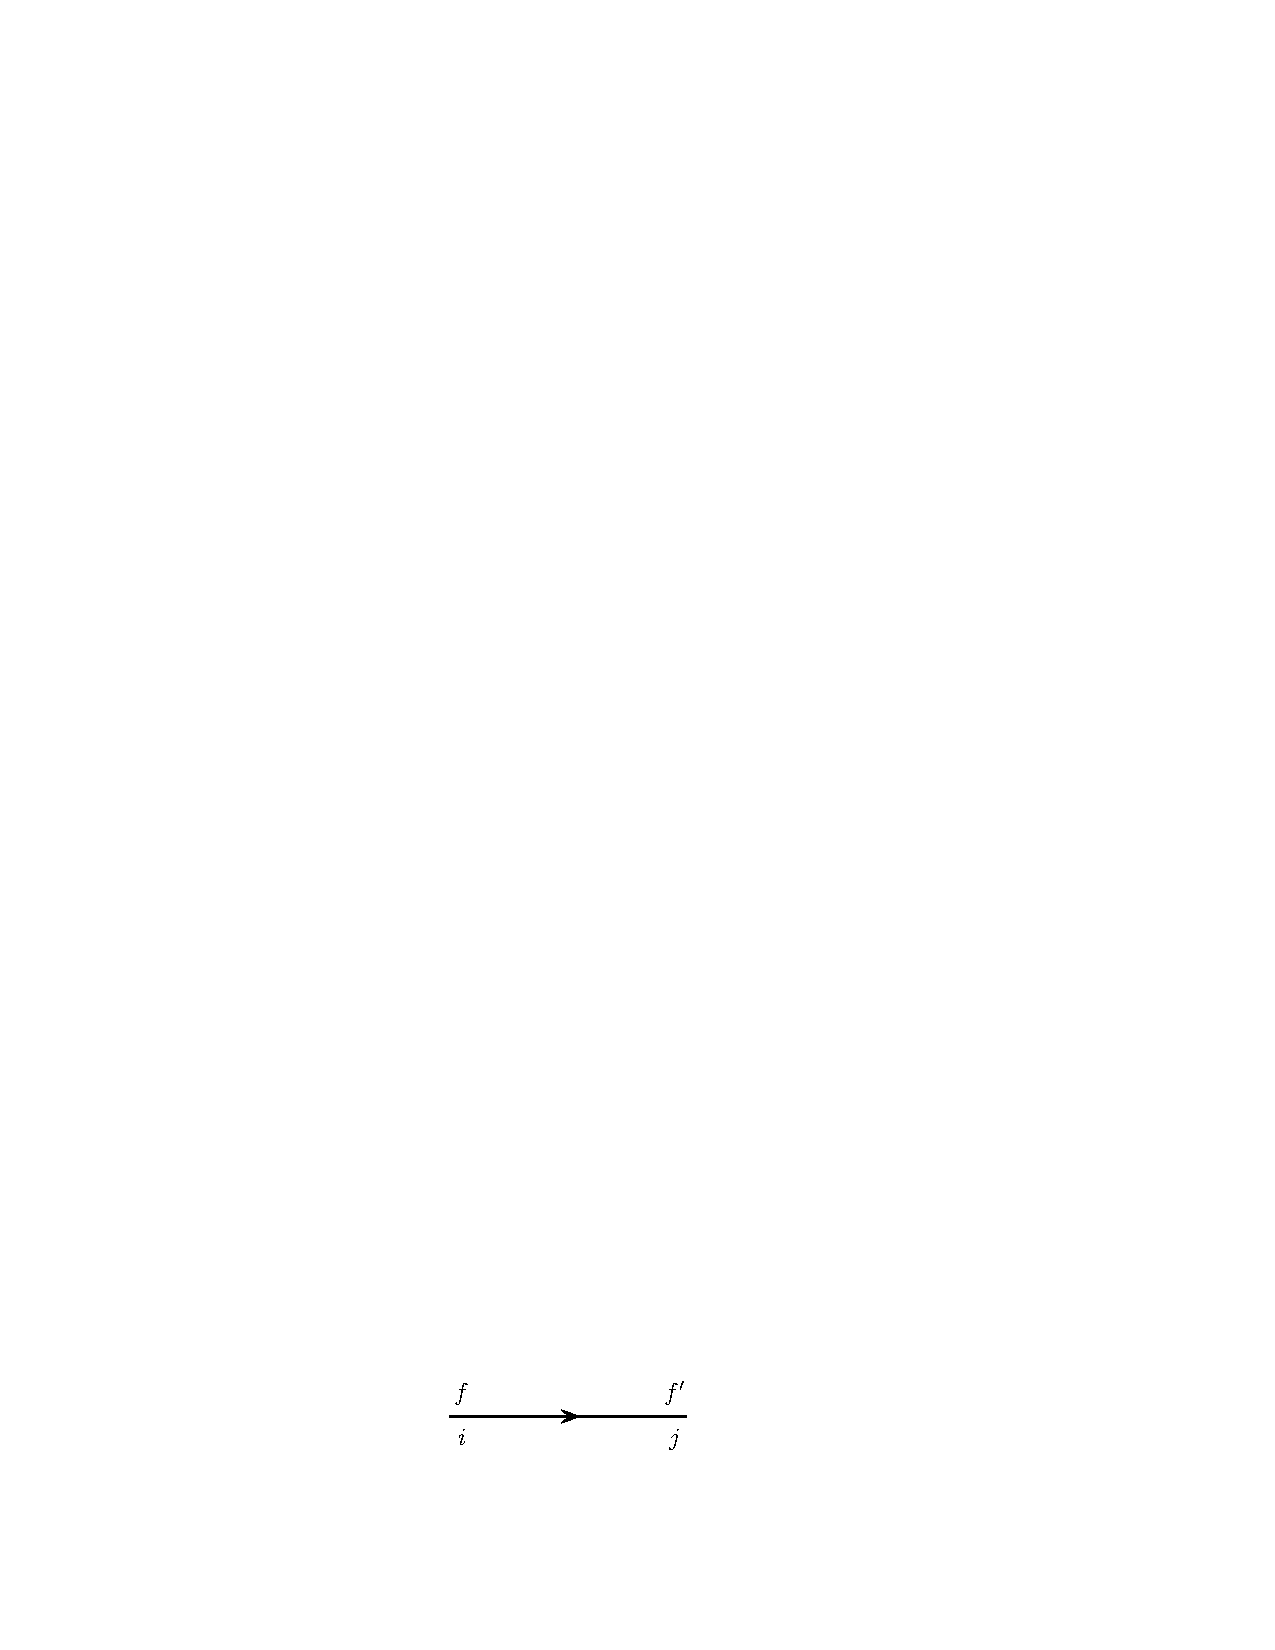
\includegraphics[width=0.5\linewidth]{quarkProp}\end{center}
				&
				\begin{center}
					\begin{equation*}
						\frac{i\delta_i^j\delta_f^{f'}(\slashed k + m)}{k^2 - m^2}
					\end{equation*}
				\end{center} \\

				\begin{center}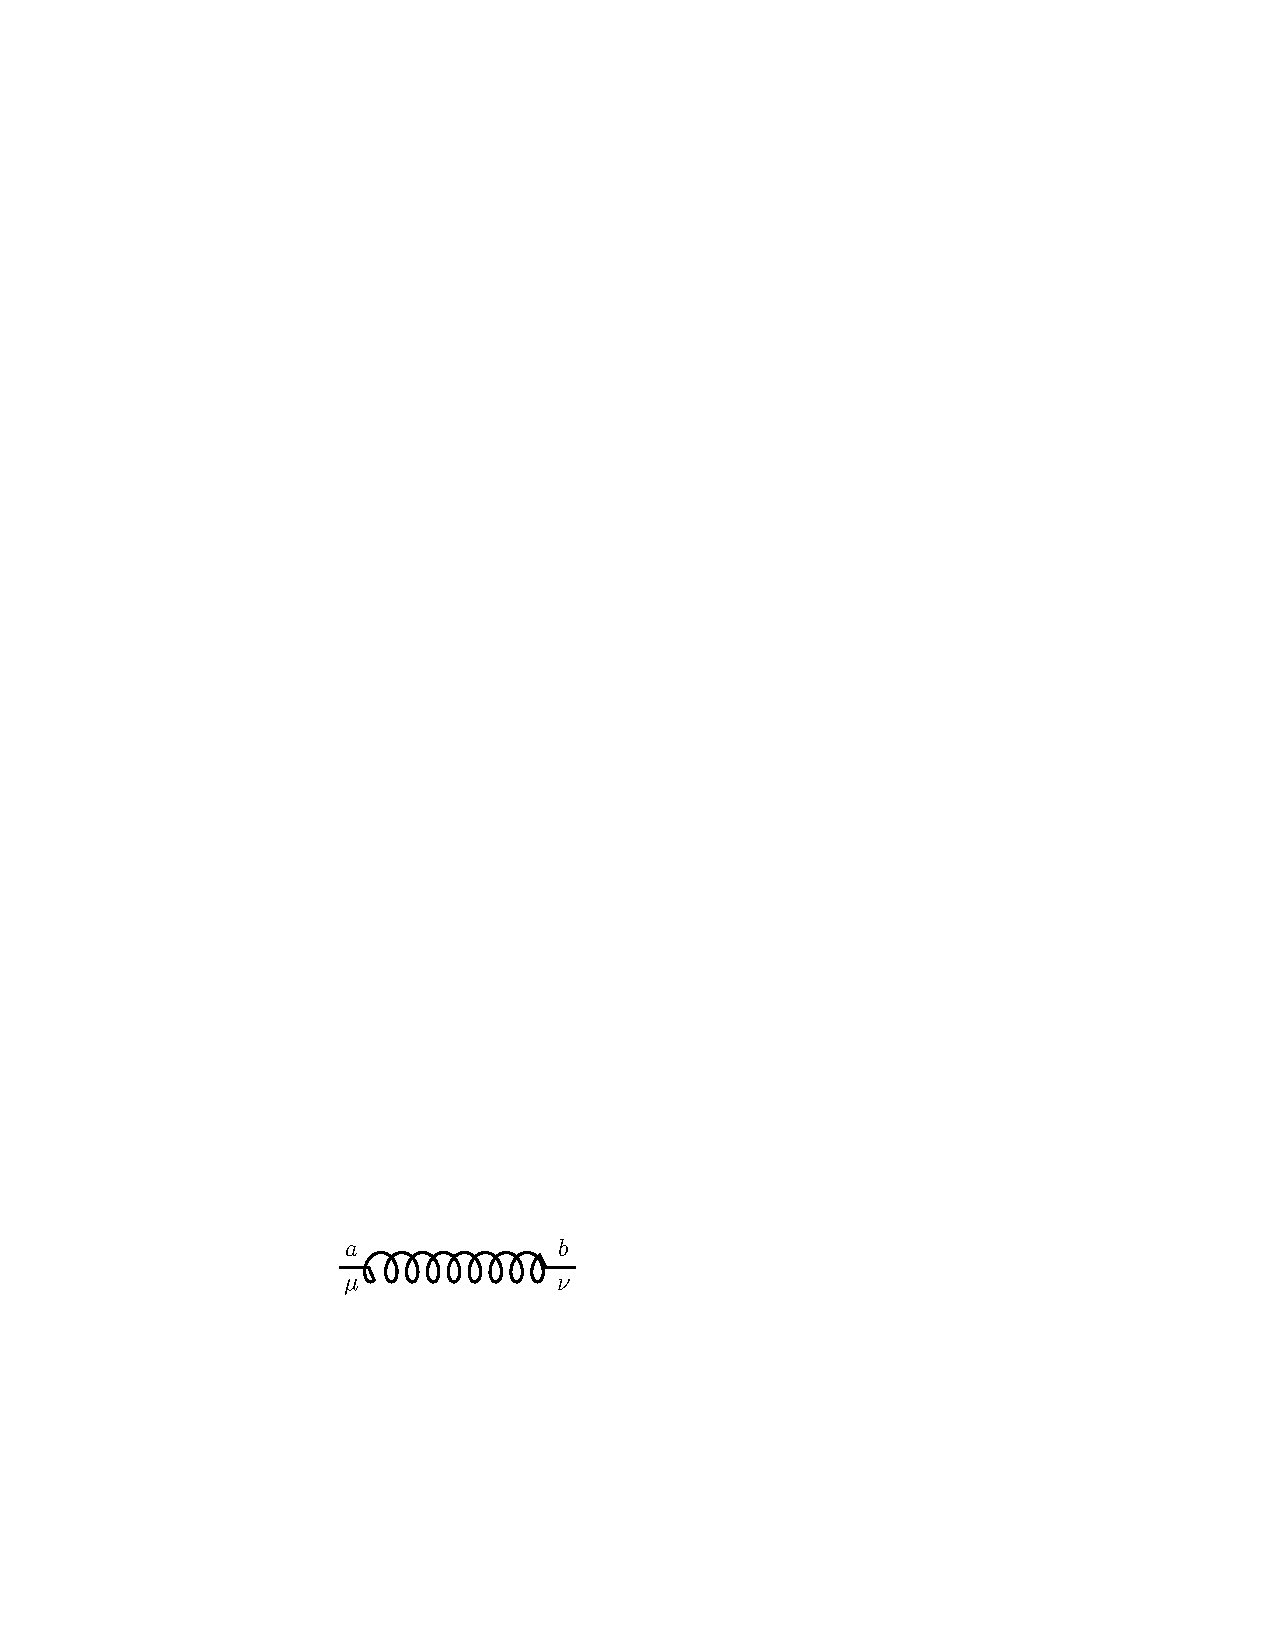
\includegraphics[width=0.5\linewidth]{gluonProp}\end{center}
				&
				\begin{center}
					\begin{equation*}
						-\frac{i\delta_a^b}{k^2}\left(g^{\mu\nu} - (\xi - 1)\frac{k^\mu k^\nu}{k^2}\right)
					\end{equation*}
				\end{center} \\

				\begin{center}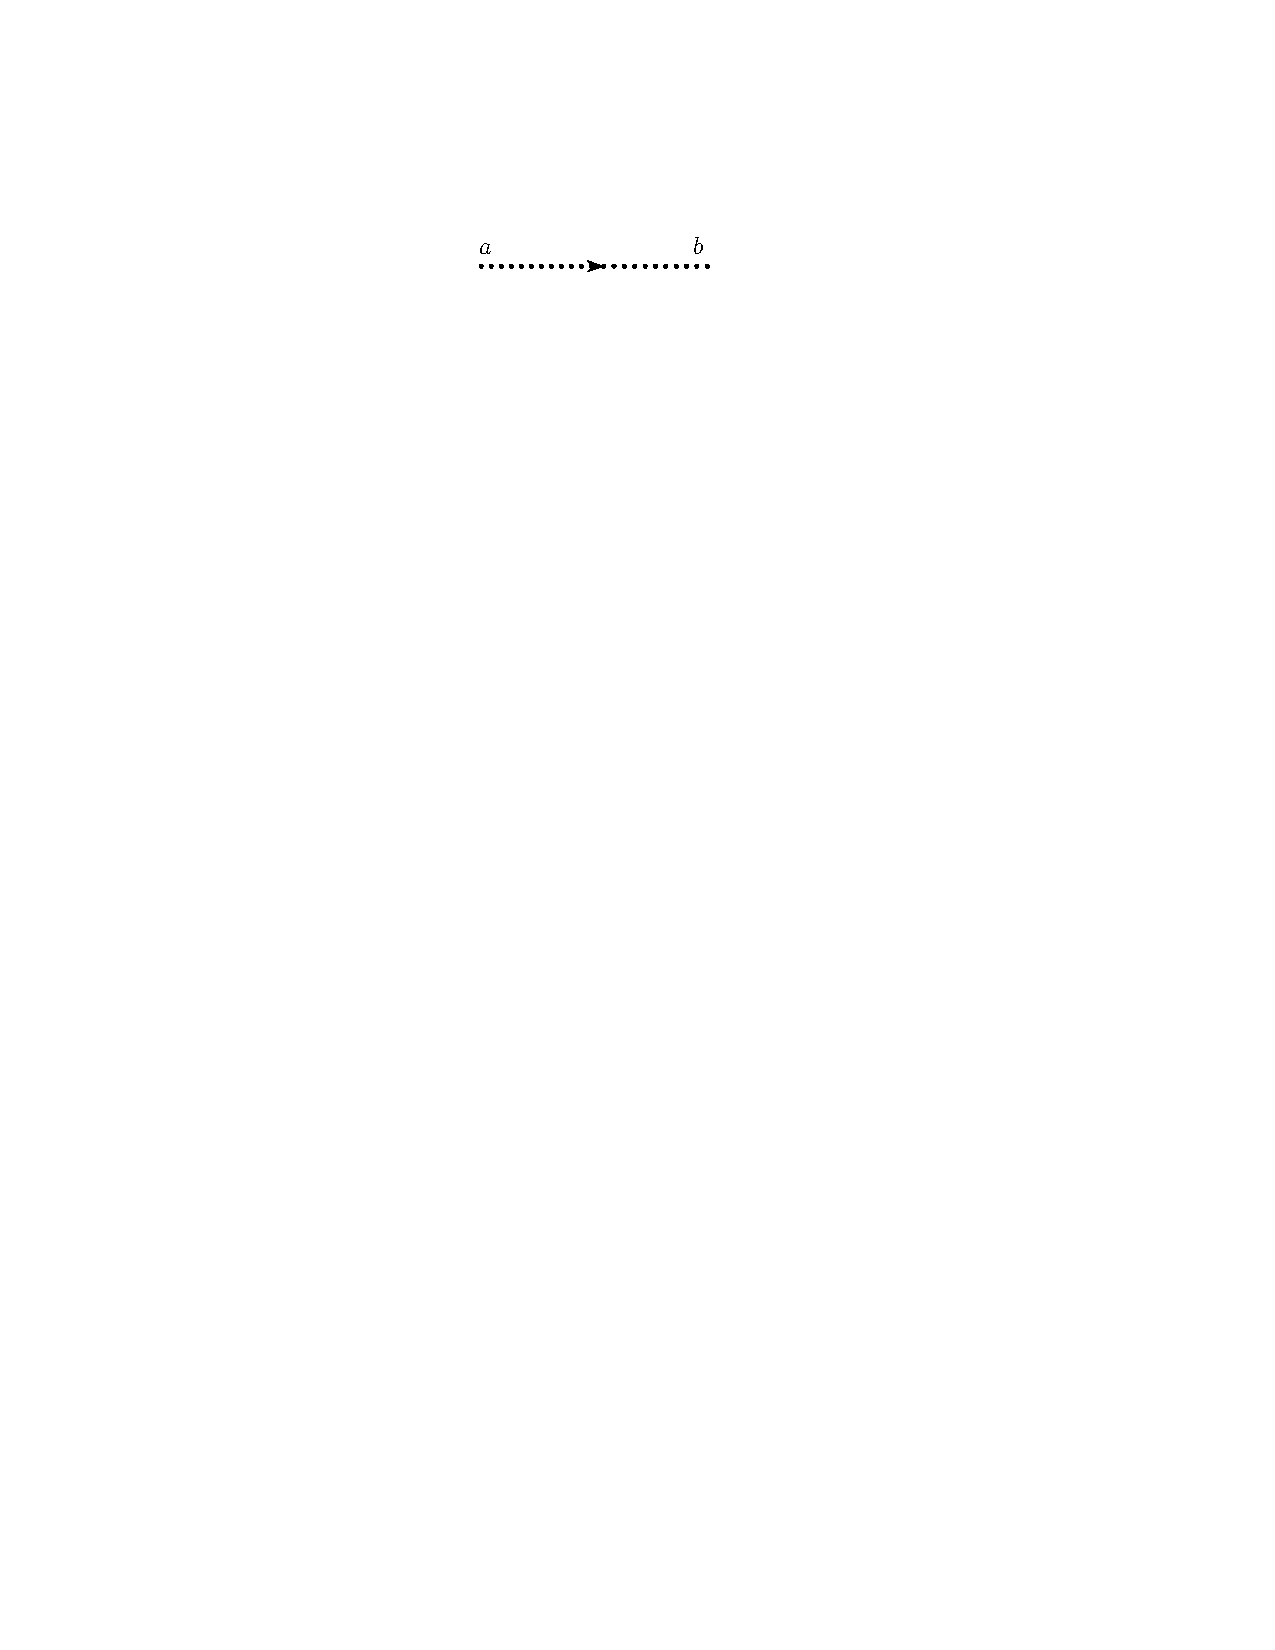
\includegraphics[width=0.5\linewidth]{ghostProp}\end{center}
				&
				\begin{center}
					\begin{equation*}
						\frac{i\delta_a^b}{k^2}
					\end{equation*}
				\end{center} \\

				\begin{center}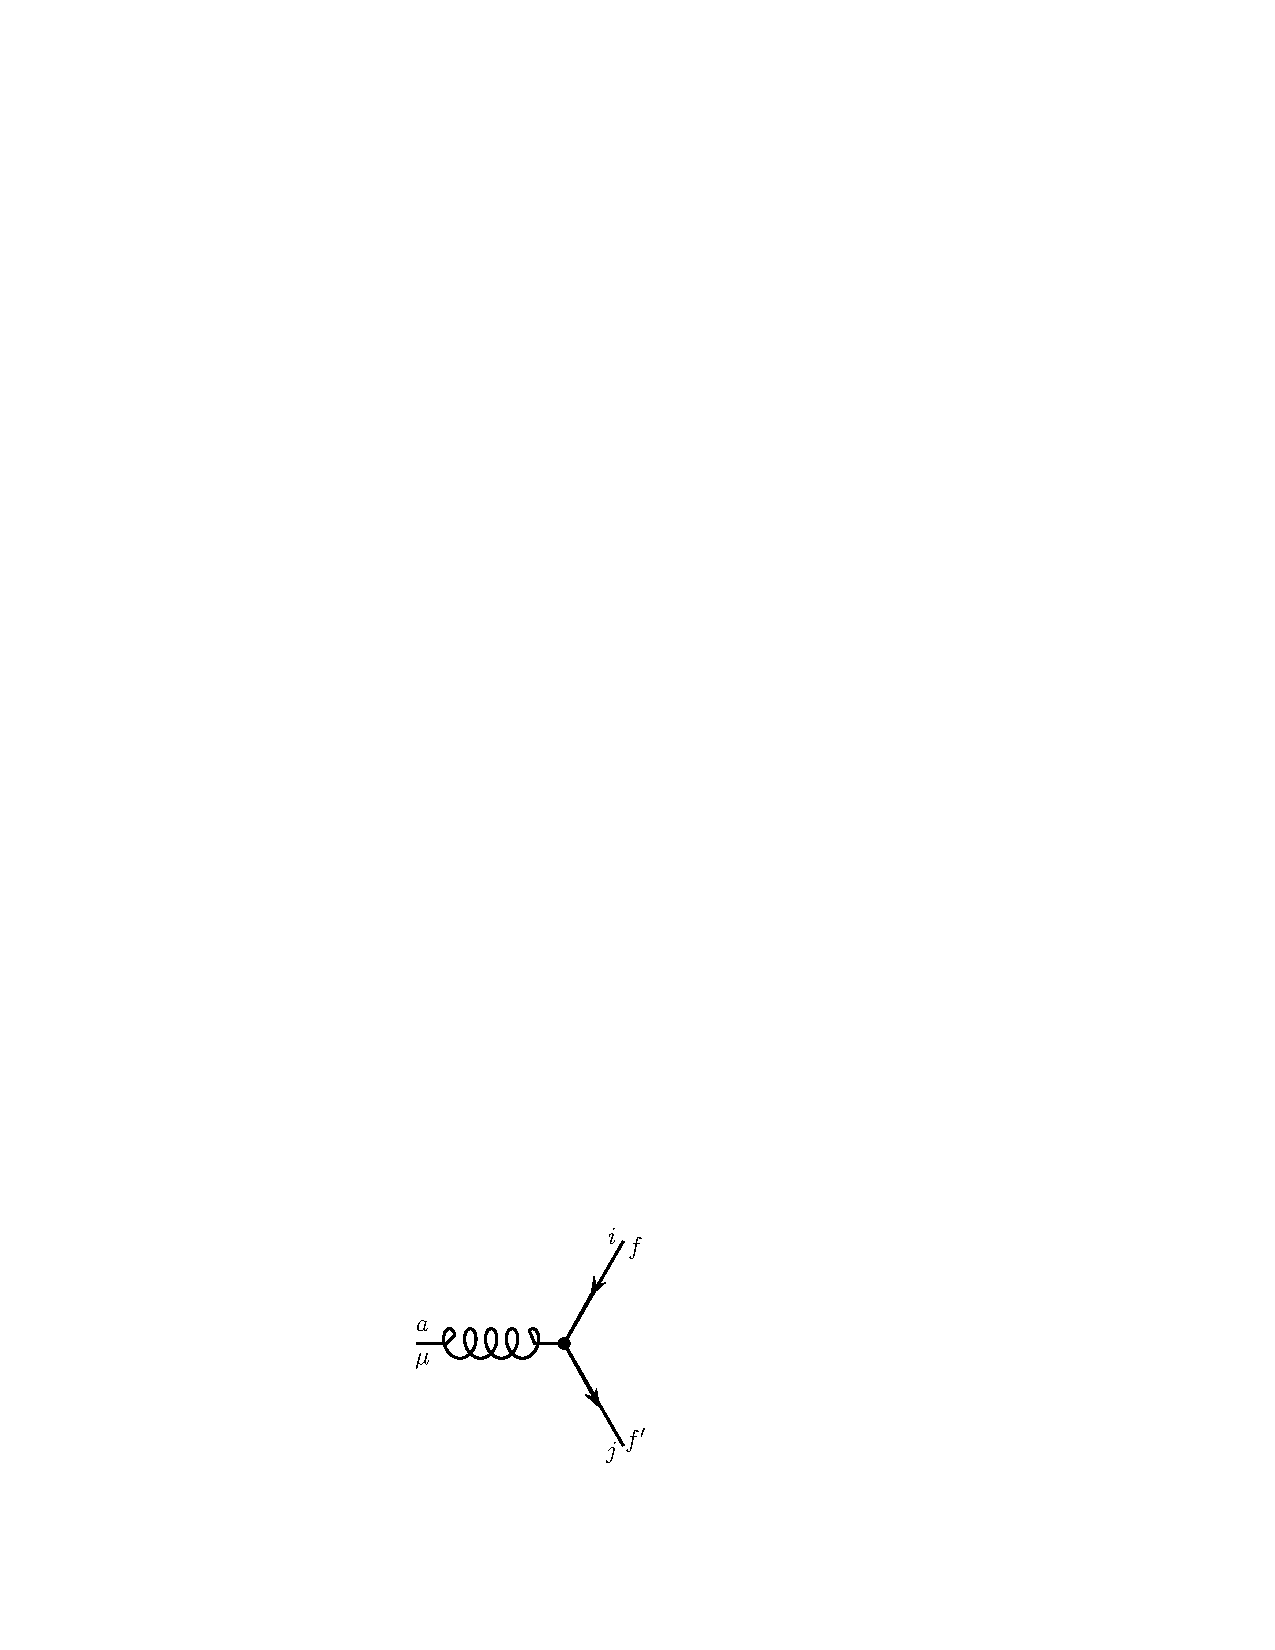
\includegraphics[width=0.40\linewidth]{qgVertex}\end{center}
				&
				\begin{center}
					\begin{equation*}
						-ig_s\gu{\mu}\delta_f^{f'}T^a_{ij}
					\end{equation*}
				\end{center} \\

				\begin{center}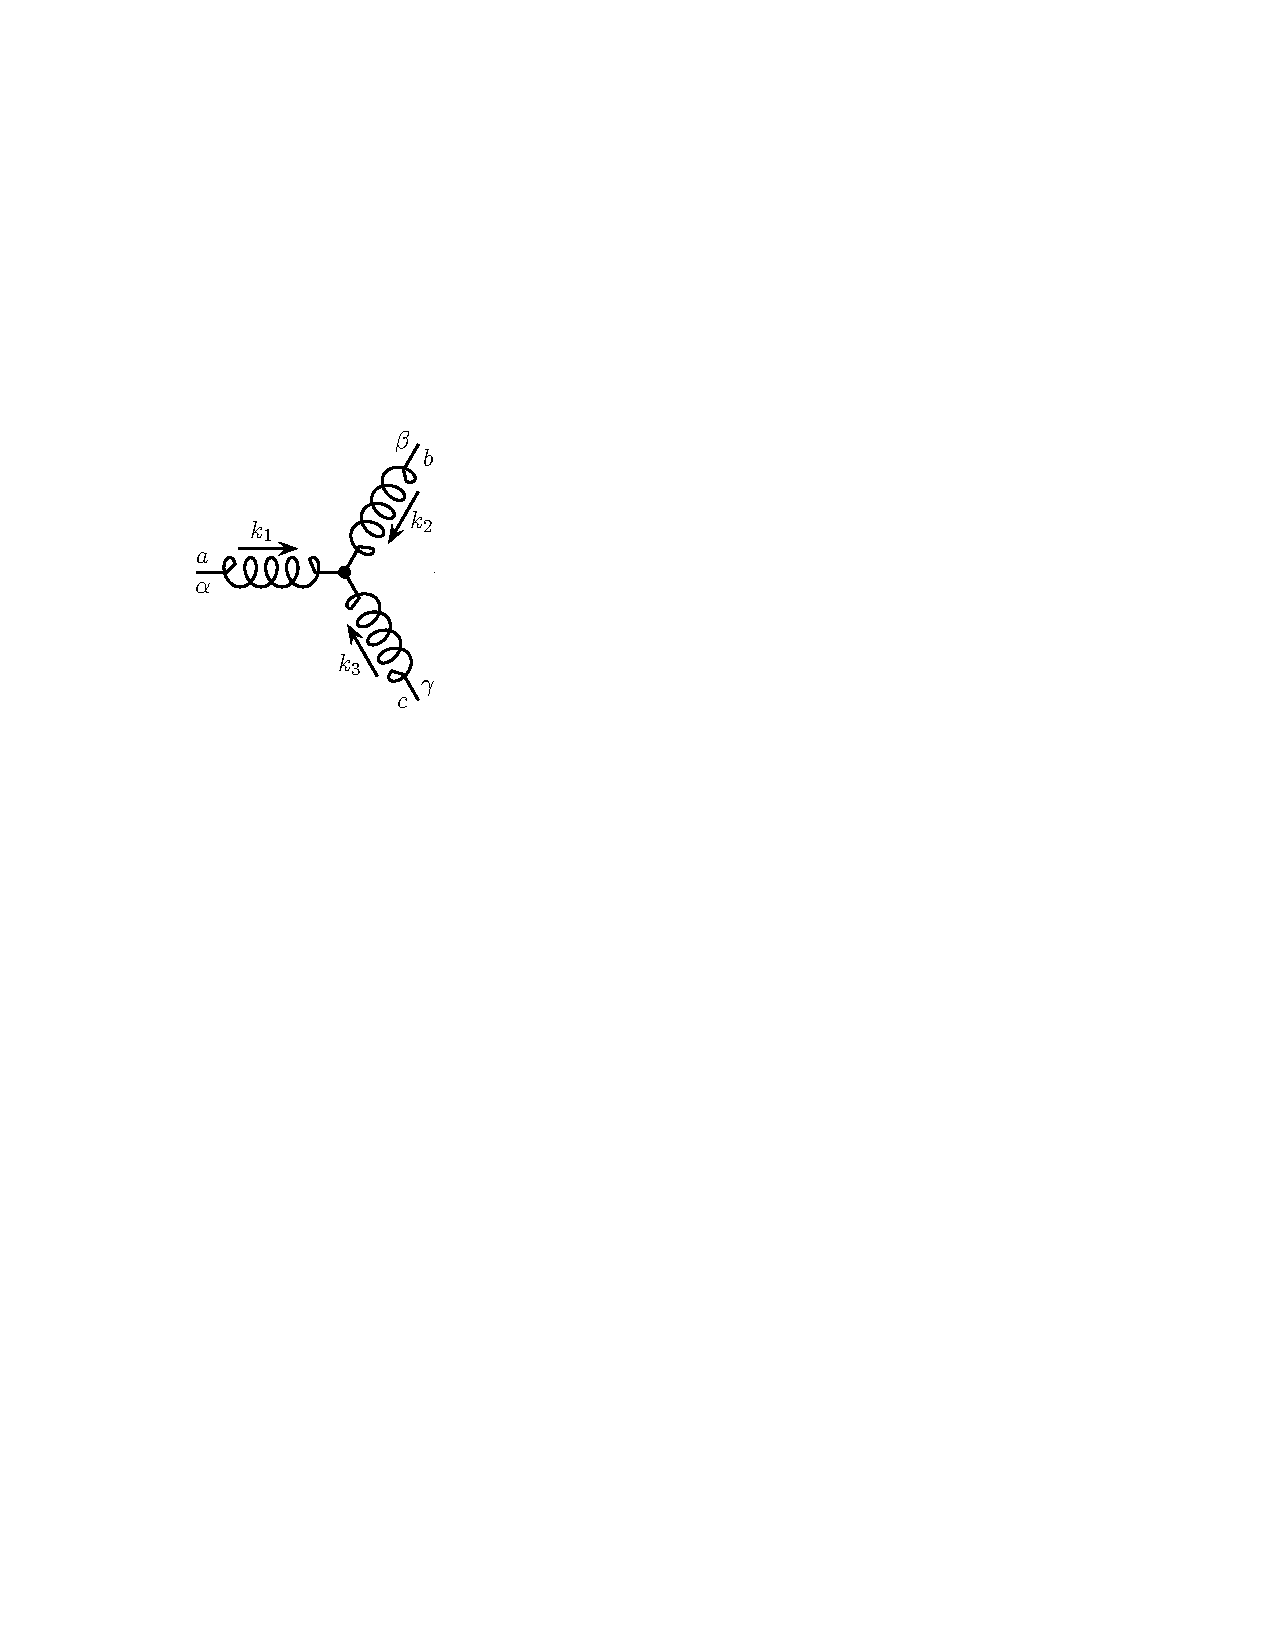
\includegraphics[width=0.40\linewidth]{tripleGluon}\end{center}
				&
				\begin{center}
					\begin{align*}
						-g_s f^{abc}\Big (g^{\alpha\beta}(k_{1} - k_{2})^{\gamma} + \\
						                  g^{\beta\gamma}(k_{2} - k_{3})^{\alpha} + \\
						                  g^{\gamma\alpha}(k_{3} - k_{1})^{\beta}\Big)
					\end{align*}
				\end{center} \\

				\begin{center}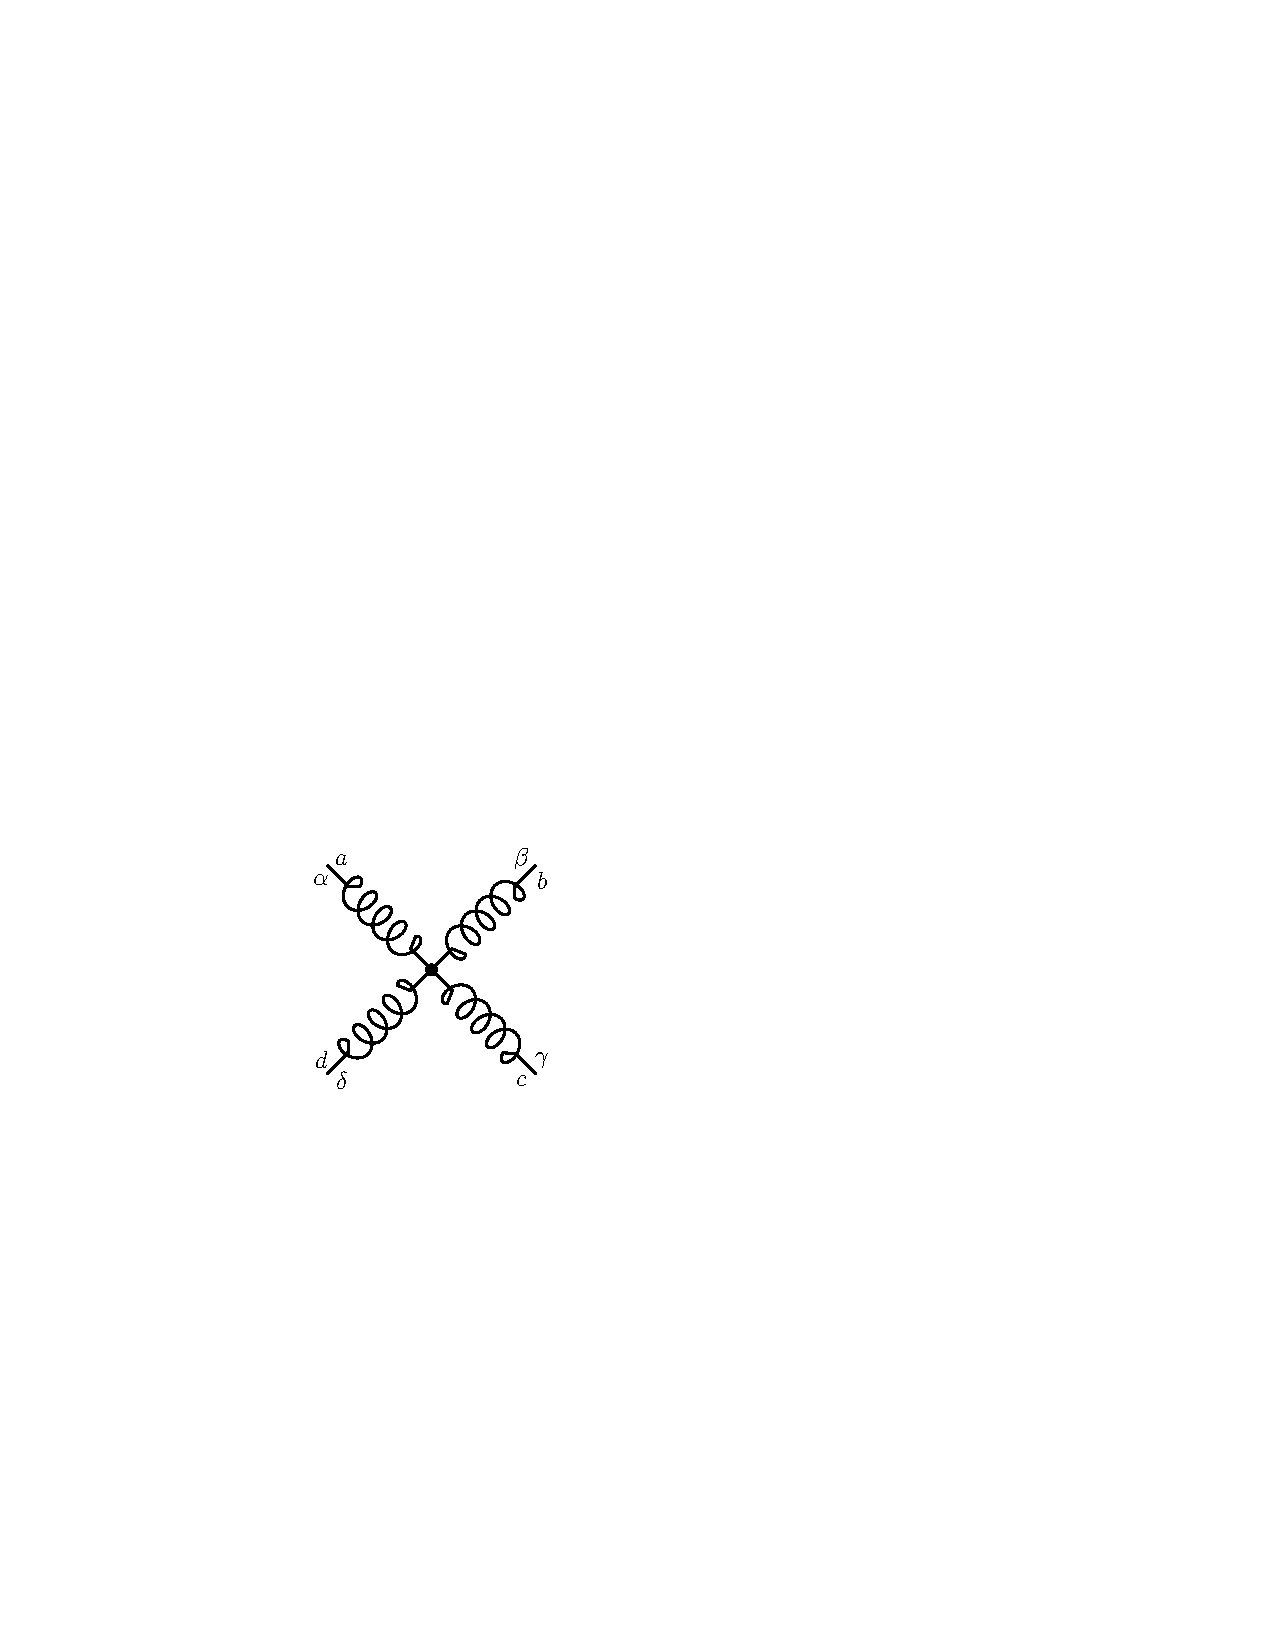
\includegraphics[width=0.40\linewidth]{quadGluon}\end{center}
				&
				\begin{center}
					\begin{align*}
						-ig_s^2\Big(f^{abe}f^{cde}(g^{\alpha\gamma}g^{\beta\delta} - g^{\alpha\delta}g^{\beta\gamma}) + \\
						            f^{ace}f^{bde}(g^{\alpha\beta}g^{\gamma\delta} - g^{\alpha\delta}g^{\gamma\beta}) +  \\
						            f^{ade}f^{bce}(g^{\alpha\beta}g^{\delta\gamma} - g^{\alpha\gamma}g^{\delta\beta})\Big) \\
					\end{align*}
				\end{center} \\

				\begin{center}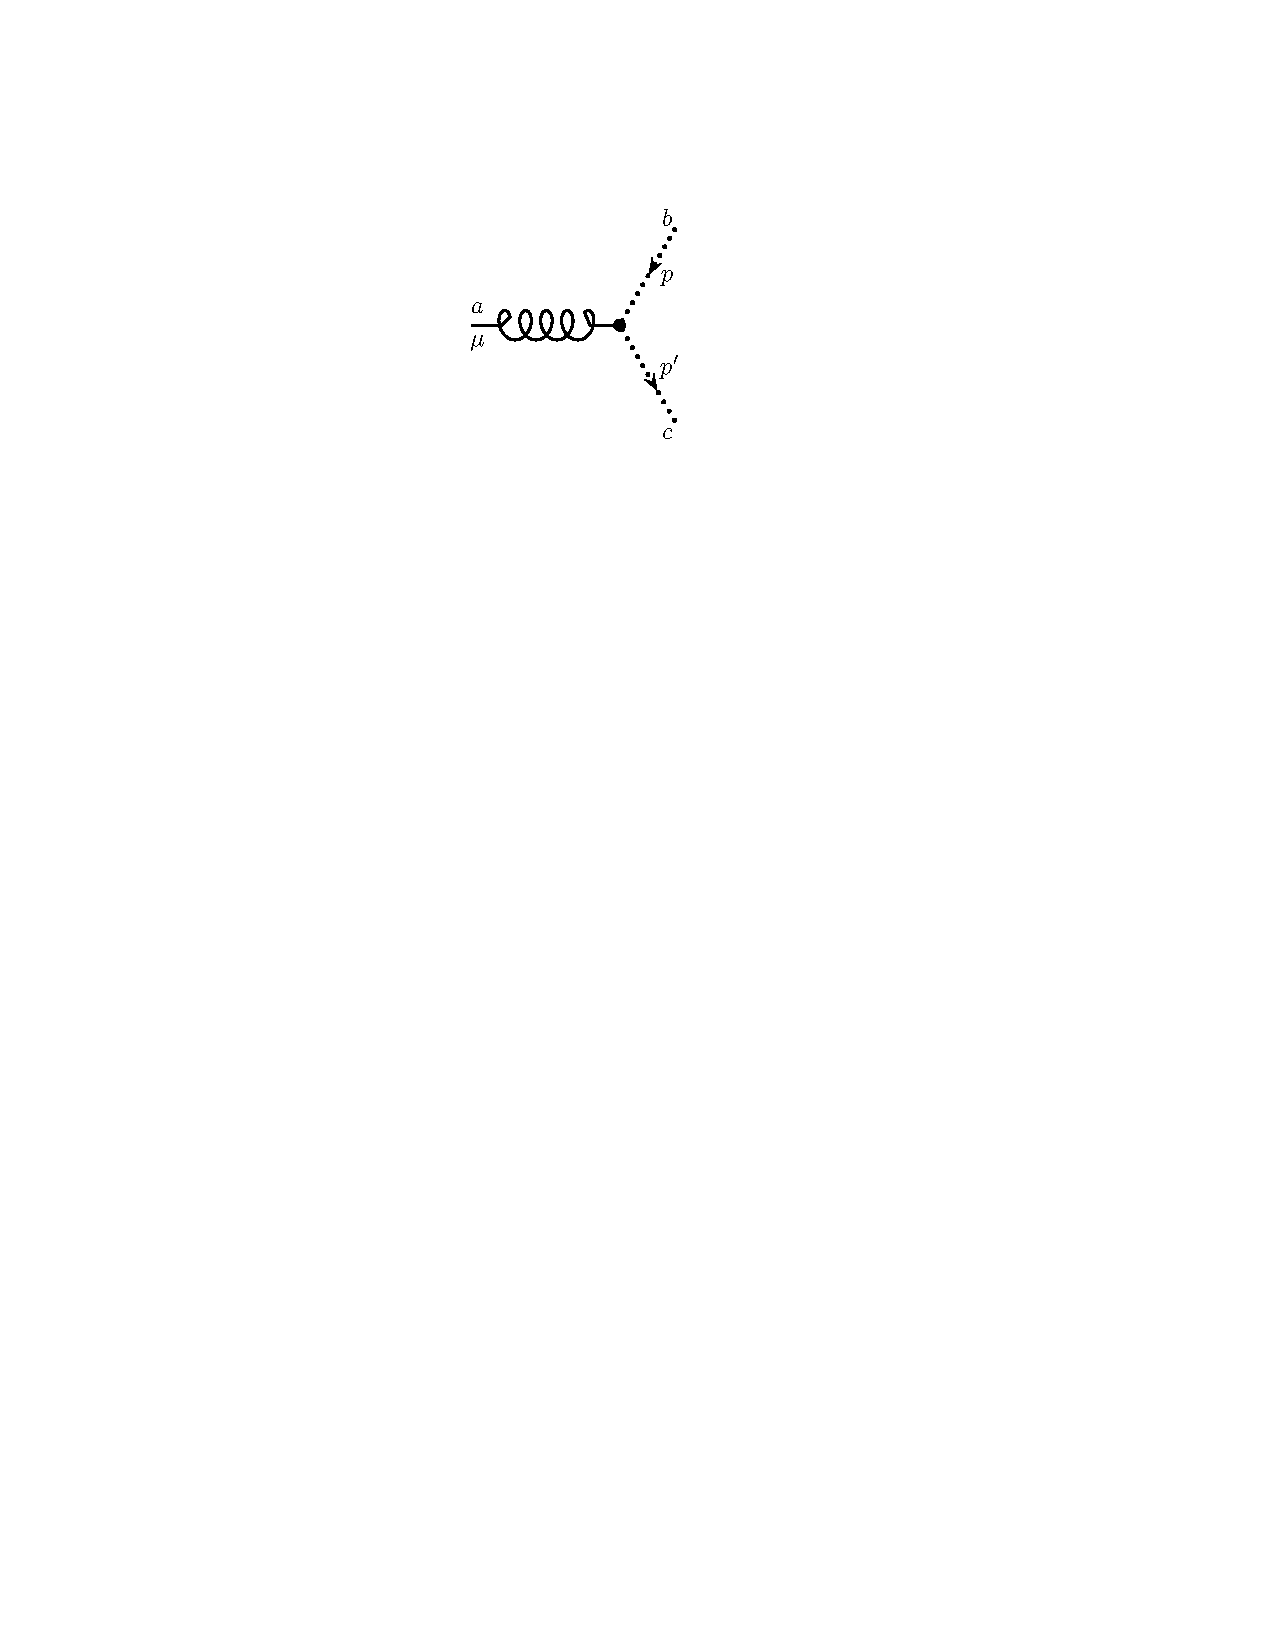
\includegraphics[width=0.40\linewidth]{gluonGhost}\end{center}
				&
				\begin{center}
					\begin{equation*}
						if^{abc}p'_{\mu}
					\end{equation*}
				\end{center} \\
			\hline
		\end{tabular}
		\label{tab:feynRules}
	\end{table}

	\begin{enumerate}
		\item Incoming external lines with spin $s$ and momentum $p$ are given a factor of $u^{(s)}_i(p)$ or
		      $\overline{v}^{(s)}_i(p)$ for quarks or anti-quarks.  Similarly outgoing external quark or
		      anti-quark lines get a factor $\overline{u}^{(s)}_i(p)$ or $v^{(s)}_i(p)$.  If the external particles
		      are not coloured the procedure is the same but of course the spinors will no longer be $SU(3)$
		      fundamental vectors.  External gluons with momentum $p$, polarisation $\epsilon$ and colour $a$ are
		      replaced by $\epsilon^a(p)$ or $\epsilon^{a*}(p)$ depending on whether they are incoming or outgoing.
		\item For each vertex or propagator in the Feynman diagram insert the corresponding mathematical
		      expression (see tab. (\ref{tab:feynRules})).  The order of the Lorentz indices must be the same
		      as that found by tracing the fermion lines in the diagram backwards,
		\item A factor of $-1$ must be included for each anti-fermion line flowing from the initial state
		      to the final state,
		\item A factor of $-1$ must be included for each fermion, anti-fermion or ghost loop in the diagram
		\item An integration over any unconstrained momenta in the diagram must be included with measure:
		      \begin{equation}
		      	\int\frac{d^4k}{(2\pi)^4},
		      \end{equation}
		      where $k$ is the momenta in question and the integral is understood to run over all four momentum
		      components form zero up to infinity,
		\item A diagram dependent symmetry factor must be included,
		\item Lastly, for an unpolarised calculation we must sum over initial spin and colour and average
		      over all possible final spins and colours.
	\end{enumerate}

	The $u(p)$ and $v(p)$ are Dirac spinors which solve the free Dirac eq. for a plane-wave:

	\begin{equation}
		(i\slashed p - m)u(p)=0\hspace{1cm}(i\slashed p + m)v(p)=0.
		\label{eqn:diracPW}
	\end{equation}

	The result of following these Feynman rules is what we refer to as the matrix element, $\mathcal{M}$.  We will now detail how
	we go from the matrix element of some scattering process to a useful physical observable: the \emph{partonic cross-section},
	$\hat{\sigma}$.  The matrix element is related to the fully-differential cross-section by `Fermi's golden rule' which, for
	a scattering process $p_{a} + p_{b}\rightarrow p_{1} + \ldots + p_{m}$ is given by

	\begin{align}
	\begin{split}
		d\hat{\sigma} = &\frac{|\mathcal{M}(p_{a} + p_{b}\rightarrow p_{1}^{(f)}, \ldots, p_{m}^{(f)})|^2}{F}\\
		\times&(2\pi)^4\delta^{(4)}(p_{a} + p_{b} - p_{1} - \ldots - p_{m}) \\
		\times&\frac{d^3\vec{p}_1}{2E_1(2\pi)^3}\cdots\frac{d^3\vec{p}_m}{2E_m(2\pi)^3},
	\end{split}
	\end{align}

	where $F=4\sqrt{(p_ap_b)^2 - m_a^2m_b^2}$ is the flux of the incoming particles and the delta function acts to
	enforce momentum conservation for the process.\\We now have a procedure for going from a scattering process
	we wish to calculate to the differential cross-section for that process.

\section{Divergences and Regularisation}
	\label{sec:divAndReg}

	In the preceding section we saw that any unconstrained momenta in a Feynman diagram must be integrated over to account
	for all possible ways the momenta in the process may flow.  We refer to these contributions as loop-level or
	higher-order corrections.  When calculating these corrections we encounter divergences of various kinds which can be
	divided up into three classes based on how they arise.

	\subsection{Ultraviolet divergences}

		Ultraviolet divergences (UV) occur when all the components of a loop momenta grow large,
		$k^\alpha\rightarrow\infty$, such that $k^2$ becomes the dominant term in propagator.
		Since these extremely high momentum modes correspond to physics at very short distance scales
		we choose to interpret these divergences as an indication that our theory is only an naive
		theory and we shouldn't attempt to apply it to all scales.  We can quickly spot diagrams with these
		pathologies with a naive power counting argument.  For example, given a diagram which results in a
		term such as the following:

		\begin{equation}
			\int \frac{d^4k}{k^2(k^2-m^2)},
		\end{equation}

		where $m$ is some finite mass. In the UV region where $k\rightarrow\infty$ this is asymptotically equal
		to:

		\begin{equation}
			\sim\int\frac{d^4k}{k^4},
		\end{equation}

		which is clearly logarithmically divergent.

	\subsection{Infrared and collinear divergences}

		Infrared and collinear divergences (IRC) occur in theories with massless gauge bosons, such as
		QED and QCD, since a particle may emit any number of arbitrarily such bosons with infinitesimal
		energy and we would never be able to detect their emission.  In contrast to the UV divergences
		the IR becomes important in the region of phase space where $k^2\rightarrow0$.  A similar power
		counting analysis to that above can be applied here.  For example if we consider the one-loop
		correction to the the vertex diagram in massless phi-cubed from section (\ref{sec:partonicCrossSection})
		we would find an integral of the form \cite{Sterman:1995fz}:

		\begin{equation}
			I = \int\frac{d^4k}{(2\pi)^4}\frac{1}{k^2(p_1-k)^2(p_2+k)^2},
		\end{equation}

		where $k$ is the loop momentum, $q=p_1+p_2$ is the incoming momentum and $p_i$ the outgoing
		momenta.  Writing each momentum in light-cone coordinates with $p_1$ in the plus-direction,
		$p_2$ in the minus-direction, such that:

		\begin{align}
			p_1 \sim (p_1^+, 0, \vec{0}) \hspace{0.75cm} p_2 \sim (0, p_2^-, \vec{0}).
		\end{align}

		and then taking the Eikonal approximation, we have:

		\begin{align}
			I &= \int\frac{dk^+k^-k^2_T}{(2\pi)^4}\frac{1}{(2k^+k^- - k_T^2)(-2p_1^+k^-)(2p_2^-k^+)},\\
			  &= \frac{1}{2q^2}\int\frac{dk^+k^-k^2_T}{(2\pi)^4}\frac{1}{(2k^+k^- - k_T^2)(-k^-)(k^+)},
			  \label{eqn:IRCscaling}
		\end{align}

		where $q^2=2p_1\cdot p_2$ since $p_i$ are massless.  Here we can further subdivide the divergences
		into a `soft' sector and a collinear one.\\Considering first the soft regime if we
		let all the components of our integration variable, $k_\mu$ become small at the same rate, that is,
		$k^\mu\sim\lambda\sqrt{q^2}$ where $\lambda\rightarrow0$ then after a change of variables equation
		\eqref{eqn:IRCscaling} becomes:

		\begin{equation}
			I \sim\int\frac{d^4\lambda}{\lambda^4},
			\label{eqn:IRdivergent}
		\end{equation}

		which diverges logarithmically for small lambda.  The collinear sector follows similarly if we now
		look at the following scaling:

		\begin{align}
			k^\pm\sim\sqrt{q^2}\hspace{0.75cm}k^\mp\sim\lambda^2\sqrt{q^2}\hspace{0.75cm}k_T^2\sim\lambda\sqrt{q^2}.
		\end{align}

		As we decrease $\lambda$ we make $k_\mu$ increasingly collinear to either $p_1$ or $p_2$.  Using
		this scaling exactly reproduces eq. \eqref{eqn:IRdivergent} and therefore is also divergent.

	\subsection{Regularising divergences}
		\label{sub:regularising}


		If we are to extract any useful information from diagrams contributing above leading-order we must find
		ways to control these divergences.  These methods are called `regularisation schemes'.  The
		general plan with all regularisation schemes is to introduce a new parameter to the calculation which
		is used to get a handle on exactly \emph{how} the integral diverges.  Once we have performed the integration
		we take the limiting case where the effect of the regulator vanishes and we will see that the divergence now
		presents itself as some singular function of the regulator.  There are
		many ways to regularise divergences each with their own advantages and disadvantages.  Here we briefly describe
		three common approaches.

		Given that the integrands seen so far only diverge in certain regions (very large or very small momenta)
		perhaps the most obvious thing to do is to manually introduced alter the limits of our integration. This
		is the momentum cut-off scheme. we simply replace the upper (lower) bound with some finite large (small)
		value, $\Lambda^2$.  This will regulate any UV (soft) divergences and allow us to complete the calculation
		provided there are no collinear singularities which this approach cannot hope to regulate.  While this
		method has the advantage of being very conceptually simple it also has the serious disadvantages of
		breaking translational and gauge invariance.  Worse still is that simply limiting the integration to
		avoid the extremities has no effect on the collinear sector.

		An alternative which \emph{does} keep both gauge and translational invariance is the Pauli-Villars
		regularisation scheme \cite{RevModPhys.21.434}.  In this picture we introduce an extra field (or many extra fields
		\cite{FROLOV1993344}) which has the opposite spin-statistics and therefore has the effect of suppressing
		the very high mass region in the integrand as follows

		\begin{equation}
			\int\frac{d^4k}{(2\pi)^4}\frac{1}{p^2-m^2}\rightarrow\int\frac{d^4k}{(2\pi)^4}\left(\frac{1}{p^2-m^2} - \frac{1}{p^2-M^2}\right),
		\end{equation}

		where $M$ is the mass of the Pauli-Villars field with $m\ll M$.  However, once again this does not treat any
		problems in the IRC sectors.  \\Lastly we have dimensional regularisation.  Here we analytically continue the
		number of dimensions in our integral away from $d=4$.  We still want to be able to return to our physical four
		dimensional theory and so we choose

		\begin{equation}
			d=4-2\epsilon
		\end{equation}

		where $\epsilon$ is the regulator by which we control the divergence. Clearly then the limit
		$\epsilon\rightarrow 0$ would recover our original theory.  It is worth noting that there are many
		conventions for defining epsilons but up to signs and factors of 2 they are equivalent. Dimensional
		regularisation treats both the UV and the IRC divergences and translational and gauge invariance are
		preserved.  The disadvantage is that this modification changes the Dirac algebra relations which
		typically makes computing the integrals more involved.\\When working in $d$ dimensions the QCD coupling
		is no longer dimensionless.  We can see this since the action is dimensionless and therefore we have

		\begin{equation}
			[\mathcal{L}] = d.
		\end{equation}

		By considering the kinetic terms of the gluon and quark fields we can see that we must have

		\begin{equation}
			[g] + 2[\psi] + [A_\mu] = d,
		\end{equation}

		and therefore

		\begin{equation}
			[g] = \frac{4-d}{2}.
		\end{equation}

		In order to artificially fix this and restore the coupling to its dimensionless state we
		introduce a scale parameter, $\mu_r$, as follows:

		\begin{equation}
			g = g_0{\mu_r}^{\frac{4-d}{2}}.
		\end{equation}

		The introduction of this scale has important consequences for our theory.  Here we follow the instructive example
		from \cite{pinkBook}.  If we have some dimensionless observable, $R$, which depends on one large scale, $Q$, which
		is much larger than all other scales in the problem (e.g. the quark masses).  One would assume that $R$ is
		approximately independent of this large scale but when we come to regulate and renormalise the divergences we have
		seen in this section the problem becomes one involving two scales and $R$ develops a dependence on the ratio of
		these scales, $\frac{Q^2}{\mu_r^2}$.  Since $\mu_r$ is completely arbitrary $R$ must be independent of it i.e if we
		now consider $R$ as a function of both the QCD coupling strength, $\alpha_s$, and the ratio of the scales we must
		have that

		\begin{equation}
			\mu_r^2\frac{\partial R}{\partial\mu_r^2} + \mu_r^2\frac{\partial \alpha_s}{\partial \mu_r^2}\frac{\partial R}{\partial\alpha_s} = 0,
			\label{eqn:chainRuleOnR}
		\end{equation}

		for convenience we define $t = \ln\frac{Q^2}{\mu_r^2}$ and $\beta(\alpha_s) = \mu_r^2\frac{\partial \alpha_s}{\partial \mu_r^2}$
		and so we can write \ref{eqn:chainRuleOnR} as

		\begin{equation}
			\frac{\partial R(e^t, \alpha_s)}{\partial t} - \beta(\alpha_s)\frac{\partial R(e^t, \alpha_s)}{\partial \alpha_s} = 0.
		\end{equation}

		This can be solved by defining the `running QCD coupling', $\alpha=\alpha(Q^2)$

		\begin{equation}
			t = \int_{\alpha_s}^{\alpha(Q^2)}\frac{dx}{\beta(x)},
			\label{eqn:solvingRunning}
		\end{equation}

		where $\alpha=\alpha(Q^2)$ admits the boundary condition $\alpha(\mu_r^2)=\alpha_s$.  Therefore the scale dependence
		of our observable $R$ comes about through its dependence on $\alpha_s$ only.

\section{The QCD Beta function}
	\label{sec:betaFunction}

	QCD has two striking features which are not apparent from the Lagrangian derived above.  The first is asymptotic freedom.
	This is the fact that at \emph{high} energies the QCD coupling strength becomes increasingly weak and it is this which allows us to
	perform a perturbative expansion of physical observables such as cross-sections.  The second feature is confinement.  Confinement
	is the reason we do not observe bare quarks and gluons in nature, instead we only see bound states of these fundamental QCD partons.
	This is because at very \emph{low} energies the coupling strength becomes increasingly strong.\\As we saw in section \ref{sec:divAndReg}
	when we renormalise QCD to remove the ultraviolet singularities we introduce a scale dependence in the coupling strength,
	$\alpha_s = \alpha_s(\mu_r)$.  It can be interpreted as a measure of our ignorance of the true high-scale theory which governs nature,
	that is to say, we believe QCD is the right theory \emph{only up to} some scale $\mu_r$.  The evolution of $\alpha_s$ with $\mu_r$ is
	given by the renormalisation group equation:

	\begin{equation}
		\mu_r^2\frac{\partial\alpha_s}{\partial \mu_r^2} = \beta(\alpha_s(\mu_r^2)),
		\label{eqn:RSFlow}
	\end{equation}

	where $\beta(\alpha_s)$ is the beta function.  It can be expanded perturbatively as a series in $\alpha_s$
	as follows:

	\begin{equation}
		\beta(\alpha_s) = -\beta_0\alpha_s\left(1 + \beta_1\alpha_s + \beta_2\alpha_s^2 + \ldots \right),
		\label{eqn:betaFunction}
	\end{equation}

	where the perturbative coefficients, $\beta_i$, can be calculated using the methods of section (\ref{sec:partonicCrossSection}).
	For example the leading order contribution, $\beta_0$, is given by:

	\begin{equation}
		\beta_0 = 11 - \frac{2n_f}{3}.
	\end{equation}

	If we truncate eq. \eqref{eqn:betaFunction} at leading-order in $\alpha_s$ then we can solve eq. \eqref{eqn:RSFlow}
	and we see that the coupling, $\alpha_s(\mu_r)$, `runs' with the following form:

	\begin{equation}
		\alpha_s(Q^2) = \frac{\alpha_s(\mu_r^2)}{1 + \alpha(\mu_r^2)\frac{\beta_0}{4\pi}\ln\frac{Q^2}{\mu_r^2}}.
		\label{eqn:runningAS}
	\end{equation}

	It is clear from this (since in the standard model we have $n_f\leq6$ and therefore $\beta_0>0$\footnote{The number of
	fermions we consider depends on the energy scale we are at. Clearly we must be at an energy larger than the mass of any
	given quark for it to be produced.  This was experimentally observed in the famous $R$-ratio where the ratio of the
	$e^+e^-\rightarrow \text{hadrons}$ cross-section to the $e^+e^-\rightarrow\mu^+\mu^-$ cross-section was investigated})
	that as $Q^2$ tends to zero the coupling strength becomes very large and at high values for $Q^2$ we see that $\alpha_s(Q^2)\rightarrow0$.
	This later limit is exactly the asymptotic freedom property of QCD and it holds even when we include the higher order
	terms we neglected in the leading-order approximation used to arrive at eq. \eqref{eqn:runningAS} \cite{Beringer:1900zz}.
	It is an essential result in that it allows us to perform perturbative expansions of observables and without this none of the
	following work would be possible.  The evolution of the strong coupling with $Q^2$ is shown in fig. (\ref{fig:runningAS}),
	it shows several extracted values of $\alpha_s$ based on six various types of experiment.  For example, the hadronic
	collider predictions include studies of the ratio of the 3-jet inclusive cross-section to the 2-jet inclusive
	cross-section as a means of finding the strong coupling \cite{Chatrchyan:2013txa}.

	\begin{figure}[htp]
		\centering
		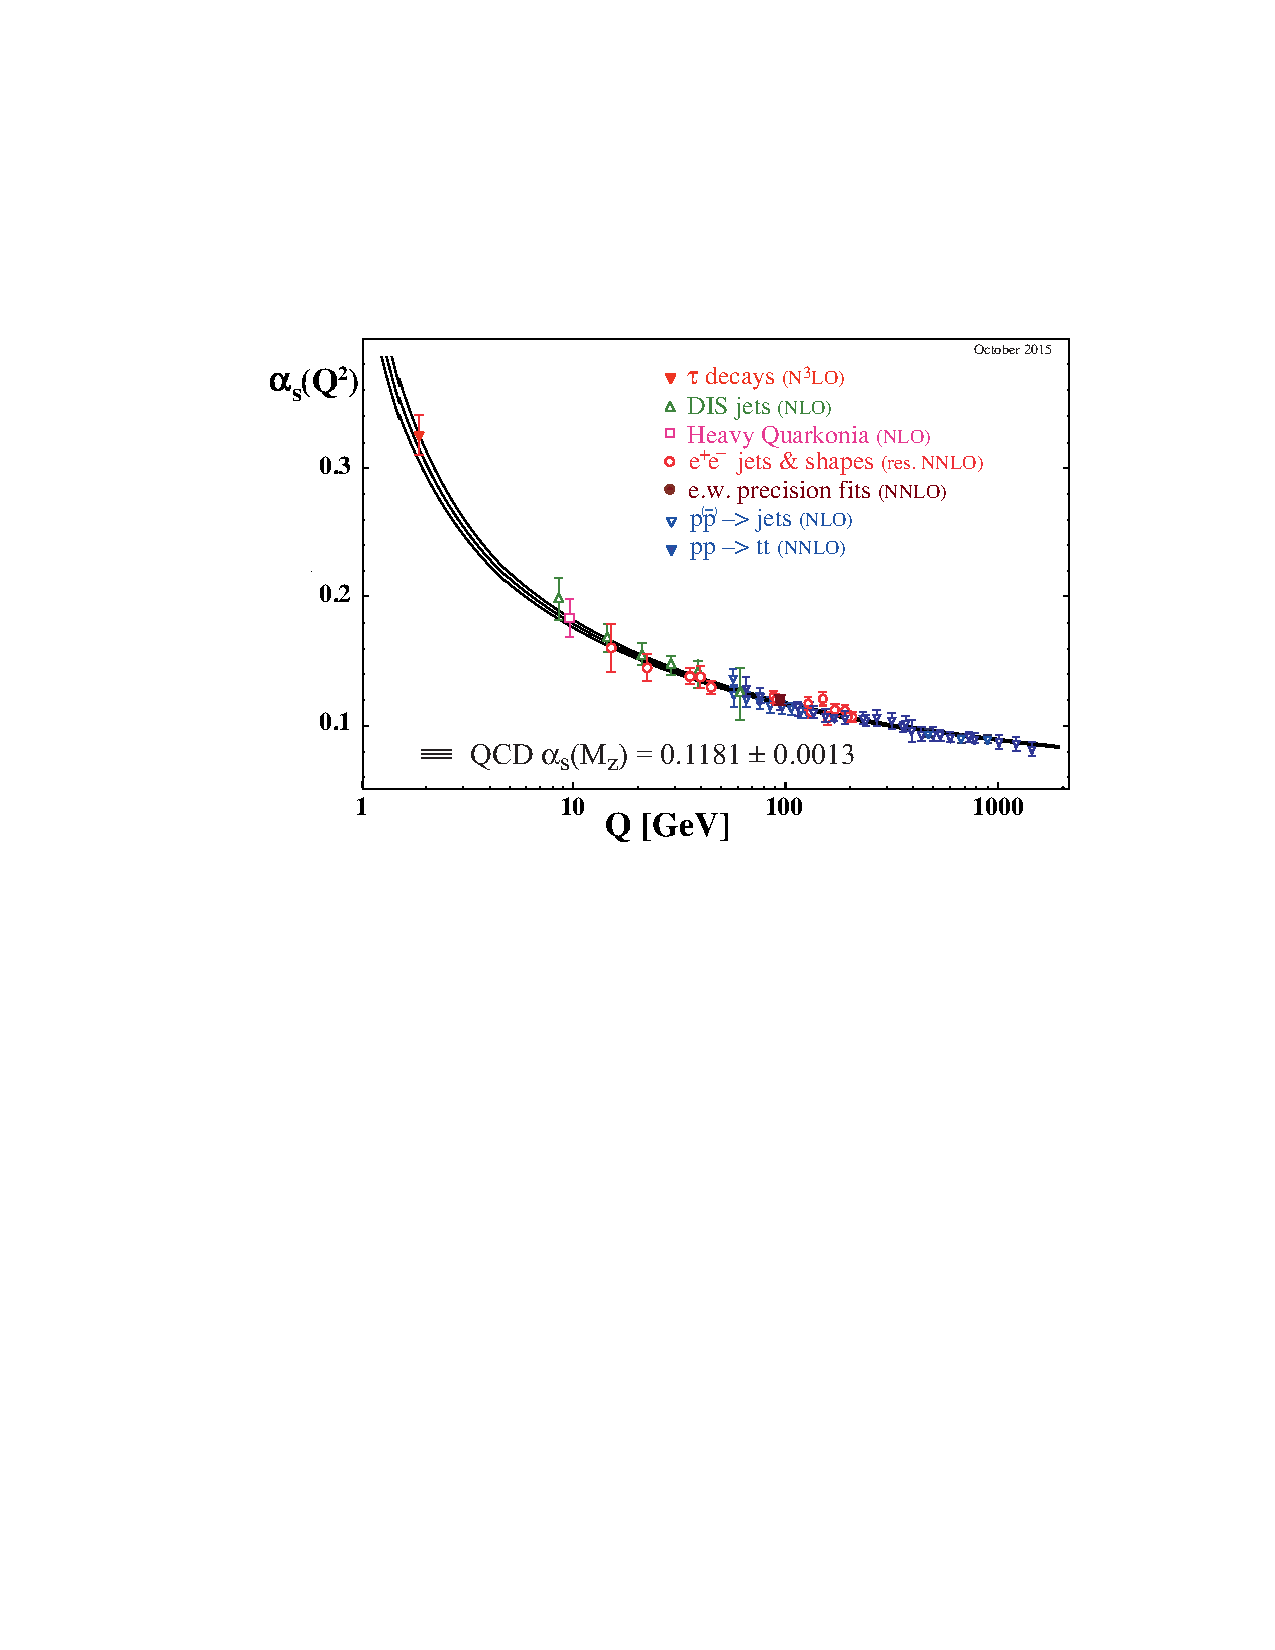
\includegraphics[width=0.9\textwidth]{Figures/runningAlphaS}
		\caption{The evolution of $\alpha_s$ over several orders of magnitude in the scale of the process $Q^2$.  The data
		         points fitted are of varying degrees of formal accuracy ranging from next-to-leading order in $\alpha_s$
		         (NLO) to next-to-next-to-next-to-leading order in $\alpha_s$ (N\textsuperscript{3}LO).
		         Fig. from \cite{Beringer:1900zz}.}
		\label{fig:runningAS}
  	\end{figure}

\section{QCD Factorisation at Hadronic Colliders}
	\label{sec:factorisation}

	So far we have only talked about the very general idea of two particles interacting and scattering off one another into
	some final state which we are interested in.  This is too simple a picture when we are considering hadronic colliders
	such as the Large Hadron Collider (proton-proton), the Tevatron (proton-antiproton), HERA (proton-lepton) and, potentially,
	a Future Circular Collider (FCC) with a hadronic initial state.\\At experiments we collide QCD bound states with one another
	but in practise when calculating cross-sections we perform a sum over the possible combinations of initial states we may
	encounter in the two incoming hadrons.  In order to do this we must have a good understanding of the dynamics of the partons
	inside the onrushing hadrons; this understanding is encoded in the Parton Distribution Functions (PDFs).  A PDF,
	$f_{i/H}(x, Q^2)$ is a function which tells us how likely we are to find a parton of type $i$ carrying a fraction $x$ of the
	total hadron's momentum in a hadron, of type $H$, during a collision occurring at an energy scale $Q$.  Because the PDFs contain
	non-perturbative information we cannot compute their properties in the same way as we calculate cross-sections, instead they
	are determined by fitting to data from a range of experiments (such as those mentioned above).  Once we have the
	PDFs we can compute the physical hadronic cross-sections, $\sigma$, by convoluting two of them (one for each hadron) with
	the partonic cross-section for the scattering of partons of type $i$ and $j$, $\hat{\sigma}_{ij}$, discussed in section
	(\ref{sec:partonicCrossSection}) and summing over the possible initial partons as follows:

	\begin{equation}
		\sigma(Q^2) = \sum_{f_a,f_b}\int_0^1dx_adx_bf_{a/H_a}(x_a, Q^2)f_{b/H_b}(x_b, Q^2)\hat{\sigma}_{ij}(\alpha_s(\mu_r), \mu_r^2, \mu_f^2).
		\label{eqn:factorisation}
	\end{equation}

	Eq. \eqref{eqn:factorisation} can be intuitively understood as a separation of scales; the long distance physics of the PDFs is
	manifestly distinct from the short distance hard scatter contained in the partonic cross-section.  The scale at which we separate the
	long and short range physics is called the \emph{factorisation scale}, $\mu_f$.  As with the renormalisation scale it is not
	\emph{a priori} clear what is the correct factorisation scale and results of perturbative calculations are often quoted with
	a `scale uncertainty' band.

\section{From Partons to Jets}

	As alluded to in section (\ref{sec:betaFunction}) the computation of scattering amplitudes can only take us so far
	when comparing simulations to experiments.  In particular, the final state quarks and gluons in our perturbative
	picture of QCD differ from the confined hadrons observed at hadronic colliders:  It is well known that final state
	QCD partons fragment and emit showers of additional radiation before finally they becomes colourless bound states
	in a process known as `hadronisation'.  This process is not perturbatively well-understood since it occurs at scale,
	often called $\Lambda_{\text{QCD}}$, at which QCD becomes non-perturbative, \emph{i.e.} the coupling constant of the
	theory has become too large for us to legitimately truncate a perturbative expansion.  There are models for both
	the `parton shower' behaviour of the energetic final state partons, such as \texttt{Pythia} \cite{Sjostrand:2007gs},
	\texttt{Herwig} \cite{Corcella:2000bw} and \texttt{Sherpa} \cite{Hoche:2014kca} as well as models for the hadronisation
	such as the `Lund string model' \cite{Andersson:2002ap} implemented in various physics software packages but most
	relevantly (for the remainder of this thesis) - in the \texttt{Ariadne} code \cite{Lonnblad:1992tz,Andersen:2011zd}.\\
	All high energy collider experiments
	see a great deal of QCD radiation in the final state.  This radiation, produced through the mechanisms outlined above,
	appears in columnated structures called `jets' and so it is at the jet level that we may compare our simulated results
	to actual measurements. The question of how we best map from the two or more parton level to the jet level is not a trivial
	one:  a single high-energy (or `hard') parton may split and form two final state jets but equally two low energy (or
	`soft') partons may combine into a single jet.\\There are several approaches to this problem include the \texttt{SISCone}
	algorithm \cite{Salam:2007xv} and Pythia's own implementation \texttt{CellJet} \cite{Sjostrand:2000wi}. However the
	most commonly user family of jet reconstruction algorithm are know as the `sequential recombination algorithms'.
	This group of approaches include the Cambridge-Aachen, $k_T$ and anti-$k_T$ algorithms. The general algorithm, as
	given in \cite{Cacciari:2008gp}, is:

	\begin{enumerate}
		\item Given a list of final state partons calculate some generalised distance, $d_{ij}$, between all possible
		      combinations of jets $i$ and $j$ as well as $d_{iB}$ where $B$ is the beam-line,
		\item We identify the smallest value of these.  If, say $d_{ab}$ is the smallest, we combine partons $a$ and $b$.
		      If however $d_{aB}$ is the smallest then we call $a$ a jet and remove it from the list of partons,
		\item We then recompute all the generalised distances and repeat steps 1 and 2 until no further partons remain,
	\end{enumerate}

	where the generalised distances are defined as

	\begin{align}
	\begin{split}
		d_{ij} &= \text{min}(k_{Ti}^{2p}, k_{Tj}^{2p})\frac{\Delta R^2}{R^2},\\
		d_{iB} &= k_{Ti}^{2p},
	\end{split}
	\end{align}

	where $k_{Ti}$ is the transverse momentum of the $i^{th}$ parton, $R$ is a free parameter in the clustering which relates
	to the size of the jets and $\Delta R^2$ is the distance in the detector metric between the two partons given by
	$\Delta R^2 = \Delta\phi^2 + \Delta y^2$ where $\Delta\phi$ and $\Delta y$ are the angular distance (about the beam line)
	between the partons and the rapidity gap between the partons respectively.  The parameter is $p$ and it is this which
	specifies precisely which clustering algorithm we are using; $p=0$ reduces to the Cambridge-Aachen scheme while
	$p=\pm1$ give the $k_T$ and anti-$k_T$ respectively.  The question of which to use is outlined in detail in
	\cite{Cacciari:2008gp} but we give a brief summary here.\\The choice of jet algorithm boils down to a handful of key
	properties the algorithm must exhibit.  Given a set of hard QCD final states we require that the result of the
	clustering algorithm, i.e. the jets and jet shapes, are not unduly sensitive to additional soft and collinear radiation.
	This is intuitively clear since, for example, a final state with a single high energy quark with momentum, $k_{Ti}$,
	may radiate infinitely a multitude of infinitely soft gluons, $k_{Ts_i}$, which may (or may not) be collinear to the
	original parton - but since $k_{Ts_i}\ll k_{Ti}$ the result must be a single jet, $j_{Ti}$, which has $j_{Ti}\sim k_{Ti}$.
	Any algorithm which satisfies this is said to be infra-red and collinear (IRC) safe.  We also want an algorithm which
	is insensitive to the hadronisation model used, or any possible extra multiple-parton or experimental pile-up emissions
	since these things are, at present, poorly understood.  It is also worth mentioning that since jet clustering algorithms
	are used in experimental triggers to quickly catagorise events they should be as computationally cheap as possible.\\Although
	the Cambridge-Aachen algorithm has advantages in some experimental searches such as studies where the substructure of
	jets is of particular interest \cite{Butterworth:2008iy, Aad:2015owa}, the most widely used sequential recombination algorithm is
	the anti-$k_t$ algorithm ($p=-1$) and so all of the work which follows and all of the experimental comparisons made will
	use this as the method for mapping simulated parton level results to a more useful set of jet level results.  The jet size
	parameter $R$ varies between experiments but is typically either 0.4 for ATLAS analyses or 0.5 for CMS analyses.

\section{Perturbative QCD and Resummation}
	\label{sec:pqcdAndResum}

	In section \ref{sec:partonicCrossSection} we saw that we could separate out the QCD Lagrangian into
	free and interacting components and that vacuum expectations of time ordered fields could be found by
	taking functional derivatives of the free partition function (eq. \eqref{eqn:fnDerviatesOfLagrangian}).
	Since terms which give rise to interactions in the Lagrangian come with a factor of the coupling strength,
	$g$, Taylor expanding the exponential in eq. \eqref{eqn:fnDerviatesOfLagrangian} will yield an infinite
	series of terms and, in principle, in order to compute any physical observable we must calculate we must
	evaluate all of these.  Of course in practise this is not possible.  We must choose a subset of terms from
	this infinite array which we reason will give the \emph{best possible approximation to the full series}.

	\subsection{Fixed-order Perturbation}

		The fixed-order perturbative approach operates on the assumption that since, as we saw in section \ref{sec:betaFunction},
		the coupling strength $\alpha_s$ in the expansion becomes small at large energy scales we may truncate the series at some
		power of $\alpha_s$.  For example given a cross-section of a scattering $X\rightarrow Y$ we wish to calculate, the fixed
		order picture of the expansion would be:

		\begin{equation}
			\sigma_{X\rightarrow Y} = \alpha_s^{i_0}(Q^2)\sum_{i=1}^N\alpha_s^{i}(Q^2)\mathcal{C}^{(i)}_{X\rightarrow Y}
		\end{equation}

		where $i_0$ accounts for processes which start above tree level and $\mathcal{C}^{(i)}_{X\rightarrow Y}$
		are the coefficient terms which encode the kinematics of the diagrams contributing at each `order'
		in the series.  Since we expect that the more terms we can calculate the better our
		truncated series will approximate the full result we should choose $N$ as large as possible though in principal
		it is determined by the complexity and the computational cost of the relevant calculation of the coefficient
		functions.  Recent progress has allowed the automation of next-to-leading order QCD calculations ($N=2$) in
		packages such in \texttt{aMC@NLO\_MadGraph} (v5) \cite{Alwall:2011uj}, \texttt{BlackHat} \cite{Bern:2012my}, \texttt{MC@NLO}
		\cite{Frixione:2010wd} and \texttt{Powheg} \cite{Frixione:2007vw}.  In general it is not known how to compute
		multi-loop (i.e. $N\geq3$) calculations and while process specific calculations have been completed
		\cite{Cacciari:2015jma, Grazzini:2015nwa, Gehrmann:2014fva}, it is still very much a hot topic in theoretical
		physics.\\It is important to note the limitations of this fixed-order scheme.  For example, if we were to consider
		NLO corrections to dijet production we would only be able to produce final states with two or three jets (since
		we can only have one extra real emission).  Clearly this is a limitation since the external fermion lines can
		radiate arbitrarily many extra gluons.  It is precisely this phenomenon which is shown in fig. 9,
		the NLO calculations (shown in green and black) are limited to $\langle jets\rangle\leq3$ which the predictions
		from \texttt{POWHEJ+PYTHIA} and \texttt{HEJ} which include higher-order corrections predict a higher average
		number of jets.  Note that the higher-order corrections here are \emph{not} the same in the case of
		\texttt{POWHEJ+PYTHIA} and \texttt{HEJ}.  Also note that although the scale uncertainty band of the NLO
		calculation \emph{does} exceed $\langle jets\rangle=3$ this is not a result of the formalism but instead comes
		about as the result of an attempt to quantify the residual dependence of the calculation on the factorisation
		and renormalisation scales.  This scale dependence of observables will be discussed in more detail in chapter
		\ref{chap:Zs}.\\There are frameworks to allow the `merging' of NLO calculations of different multiplicity.  A
		comprehensive review of such methods may be found in \cite{Alwall:2007fs}.

		We now present an instructive fixed-order calculation of the next-to-leading corrections to quark-antiquark pair
		production via an off-shell photon \cite{fieldBook}.

		\begin{figure}[hbt]
			\centering
			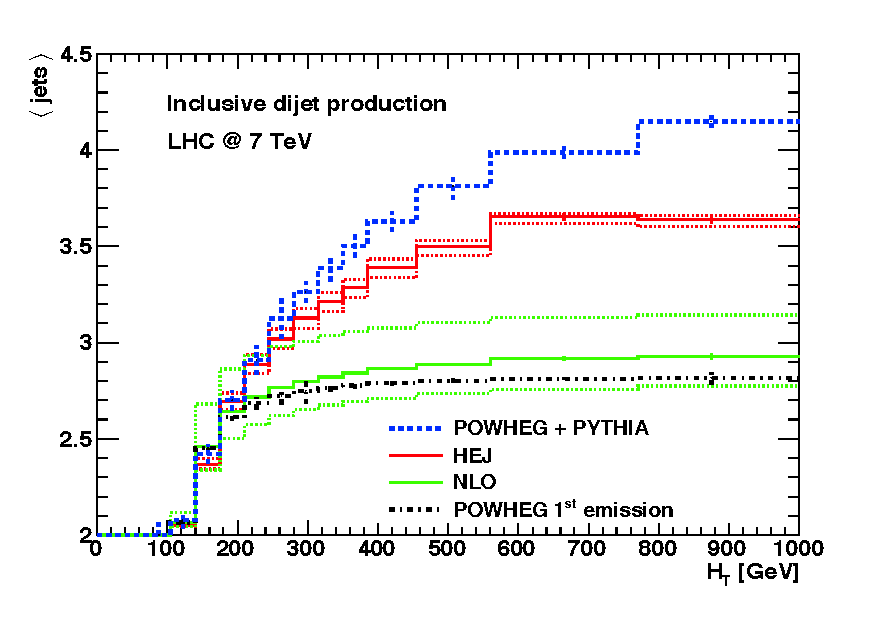
\includegraphics[width=\textwidth]{NLOfail}
			\caption{Simulations of the average number of jets as a function of the sum of the transverse momenta in the event, $H_T$,
			         for inclusive dijets at a 7TeV LHC.}
			\label{fig:NLO3jets}
  		\end{figure}

	\subsection{An Example Fixed-Order Calculation}
		\label{sub:eg1loop}

		\begin{figure}[tpb]

			\centering

			\begin{subfigure}[b]{0.48\textwidth}
				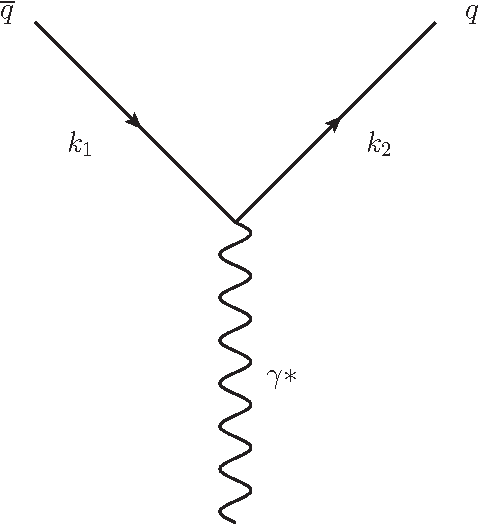
\includegraphics[width=0.8\textwidth]{TreeLevel}
				\caption{$\mathcal{A}_0$}
				\label{fig:NLOfig_1}
			\end{subfigure}
			\begin{subfigure}[b]{0.48\textwidth}
				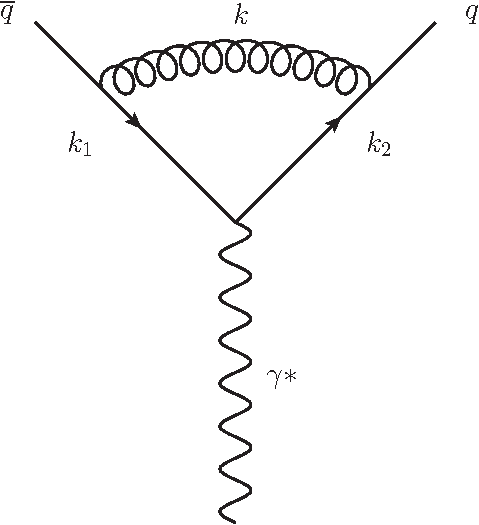
\includegraphics[width=0.8\textwidth]{NLOVirtual}
				\caption{$\mathcal{A}_v$}
				\label{fig:NLOfig_2}
			\end{subfigure}
			\begin{subfigure}[b]{0.48\textwidth}
				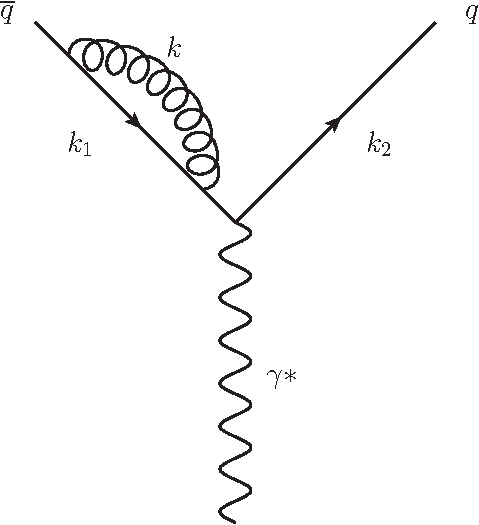
\includegraphics[width=0.8\textwidth]{NLOSelfEnergyLeft}
				\caption{$\mathcal{A}_{se1}$}
				\label{fig:NLOfig_3}
			\end{subfigure}
			\begin{subfigure}[b]{0.48\textwidth}
				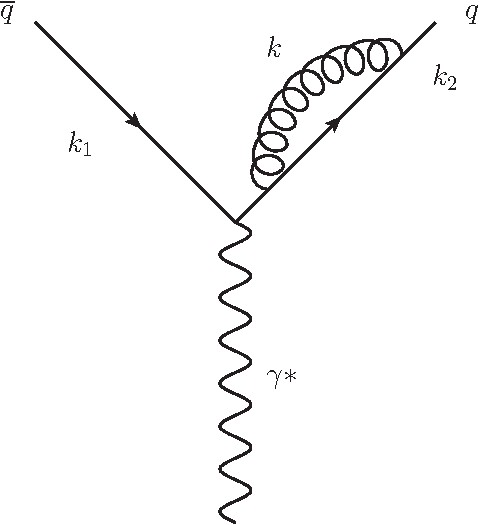
\includegraphics[width=0.8\textwidth]{NLOSelfEnergyRight}
				\caption{$\mathcal{A}_{se2}$}
				\label{fig:NLOfig_4}
			\end{subfigure}
			\begin{subfigure}[b]{0.48\textwidth}
				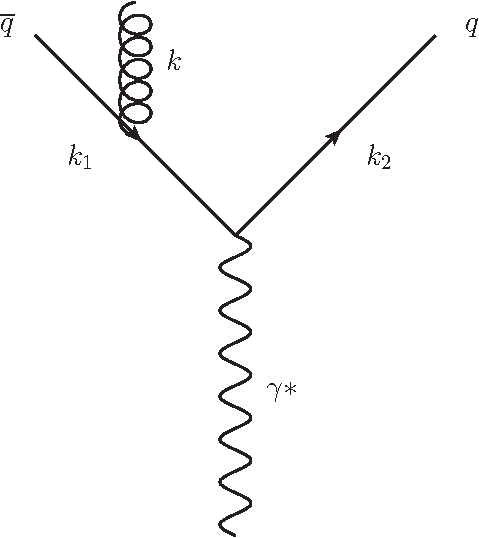
\includegraphics[width=0.8\textwidth]{NLORealLeft}
				\caption{$\mathcal{A}_{r1}$}
				\label{fig:NLOfig_5}
			\end{subfigure}
			\begin{subfigure}[b]{0.48\textwidth}
				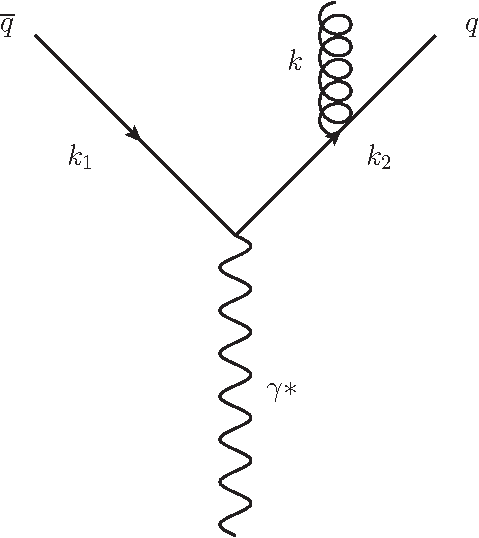
\includegraphics[width=0.8\textwidth]{NLORealRight}
				\caption{$\mathcal{A}_{r2}$}
				\label{fig:NLOfig_6}
			\end{subfigure}

			\caption{Feynman diagrams for calculating the $O(\alpha_s)$ correction to $\gamma^*\rightarrow q\overline{q}$.
			Fig. (\ref{fig:NLOfig_1}) is the leading order contribution.  Figs. (\ref{fig:NLOfig_2} - \ref{fig:NLOfig_4})
			are the virtual corrections and lastly figs. (\ref{fig:NLOfig_5} - \ref{fig:NLOfig_6}) are the real emission
			contributions.}
			\label{fig:NLOContributions}

		\end{figure}

		The Feynman diagrams which need to be included for the and $\mathcal{O}(1)$ and $\mathcal{O}(\alpha_s)$ corrections to the
		$\gamma^*\rightarrow q\overline{q}$ process are shown in fig. (\ref{fig:NLOContributions}).  We refer to fig. (\ref{fig:NLOfig_1}) as the tree level diagram,
		fig. (\ref{fig:NLOfig_2}) as the vertex correction and figs. (\ref{fig:NLOfig_3}) and (\ref{fig:NLOfig_4}) as the self-energy corrections.
		Figs. (\ref{fig:NLOfig_5}) and (\ref{fig:NLOfig_6}) are the `real corrections'.  Since the virtual corrections all have the same final state
		they must be summed and squared together.  To make the order of each term in the perturbative expansion clear we extract the $\alpha_s$
		factors from the $\mathcal{A}_i$ here.  Therefore:

		\begin{equation}
		\begin{split}
			|\mathcal{M}|^2 = &|\mathcal{A}_0 + \alpha_s\mathcal{A}_v + \alpha_s\mathcal{A}_{se1} + \alpha_s\mathcal{A}_{se2}|^2 + \mathcal{O}(\alpha_s^2) \\
			                = &|\mathcal{A}_0|^2 + 2\alpha_s\Re\{\mathcal{A}^*_0\mathcal{A}_v\} + 2\alpha_s\Re\{\mathcal{A}^*_0\mathcal{A}_{se1}\} \\
			                  & + 2\alpha_s\Re\{\mathcal{A}^*_0\mathcal{A}_{se2}\} + \mathcal{O}(\alpha_s^2),
			\label{eqn:MEBreakdown}
		\end{split}
		\end{equation}

		We can see then that to $\mathcal{O}(\alpha_s)$ we have four contributions to consider, but the two self-energy contributions will have
		the same functional form so it would seem that in practice we only need to perform three calculations - it turns out this is not the
		case; we will find that the divergence associated with exchanging a soft gluon in fig. (\ref{fig:NLOfig_2}) can only be cancelled
		if we also include the soft divergences that arise from figs. (\ref{fig:NLOfig_5}) to (\ref{fig:NLOfig_6}).  At first glance this
		seems very peculiar since these diagrams have different final states and therefore should have no business contributing to this
		calculation.  However, since the gluon can be emitted with vanishingly small momentum it would be experimentally impossible to
		detect and therefore the final states would look the same to an imperfect observer.\\It is the cancellation of these divergences
		that will be shown in detail in the next two sections.  Figs. (\ref{fig:NLOfig_1}), (\ref{fig:NLOfig_2}) and (\ref{fig:NLOfig_5})
		will be calculated in detail while the result for the self energy expressions will be omitted since it can be cancelled by
		choosing to work in the Landau gauge~\cite{fieldBook}.  Since we expect both UV and IR divergences we choose to work in the dimensional
		regularisation scheme.

		\subsubsection{The Leading Order Process}

			If we let the pair-produced quarks have charge $\pm Qe$ then the Feynman rules outlined in section \ref{sec:partonicCrossSection} give:

			\begin{equation}
				\mathcal{A}_0 = -ieQ\overline{u}^{\lambda_2}(k_2)\gamma^\mu v^{\lambda_1}(k_1)\epsilon^r_\mu(p),
			\end{equation}

			where we have used the QED Feynman rule for a quark-antiquark-photon vertex: $iQe\gamma^\mu$, the $\lambda_i$'s are the
			spins of the quarks, $r$ is the polarisation of the incoming photon and $p = k_1 + k_2$ is the momentum carried by the
			incoming photon.  To calculate we can square and since we are typically interested in unpolarised calculations we perform
			a sum over all polarisations and spins (we also choose this point to include the sum over the possible colour states of
			the outgoing quarks):

			\begin{equation}
				|\overline{\mathcal{A}_0}|^2 = 3\sum_{\forall\lambda, r}e^2Q^2[\overline{u}^{\lambda_2}(k_2)\gamma^\mu
				v^{\lambda_1}(k_1)][\overline{v}^{\lambda_1}(k_1)\gamma^\nu v^{\lambda_2}(k_1)]\epsilon^r_\mu(p)\epsilon^r_{*\mu}(p).
			\end{equation}

			We can now use Casimir's trick ~\cite{griff} to convert this spinor string into a trace, using the replacements
			$\sum_r\epsilon^r_\mu\epsilon^r_{*\nu}=-g_{\mu\nu}$ and the completeness conditions for spinors:

			\begin{equation}
				|\overline{\mathcal{A}_0}|^2 = - e^2Q^2\Tr[\slashed k_2\gamma^\mu\slashed k_1\gamma_\mu],
			\end{equation}

			where we have used the high energy limit to discard the quark mass terms.  This trace can be evaluated in arbitrary
			dimensions to give, in the high energy limit:

			\begin{equation}
				|\overline{\mathcal{A}_0}|^2 = 6e_d^2Q^2s(d-2),
			\end{equation}

			where we have defined the usual Mandelstam variable $s=(k_1+k_2)^2=2k_1\cdot k_2$ and define $e_d^2=e^2\mu^{4-d}$ where
			$\mu$ has units of mass in order to make the coupling $e$ dimensionless.  To find the leading order cross-section we divide by the
			particle flux and multiply by the two particle phase space which is given by:

			\begin{equation}
				\int d^{2d-2}R_2 = 2^{1-d}\pi^{\frac{d}{2}-1}\frac{\Gamma(\frac{d}{2}-1)}{\Gamma(d-2)}s^\frac{d-4}{2},
			\end{equation}

			where $R_2$ is the two particle phase space in $d$ dimensions.  Combining these factors and defining $\alpha_e=\frac{e^2}{4\pi}$:

			\begin{equation}
			\begin{split}
				\sigma_0 &= 3\cdot2^{2-d}\pi^{1-\frac{d}{2}}\frac{\Gamma(\frac{d}{2}-1)}{\Gamma(d-2)}s^\frac{d-4}{2}4\pi\alpha\mu^{d-4}Q^2s(d-2)\frac{1}{2s} \\
				&= 3\alpha Q^2\left(\frac{s}{4\pi\mu^2}\right)^{\frac{d}{2}-2}\left(\frac{d}{2}-1\right)\frac{\Gamma(\frac{d}{2}-1)}{\Gamma(d-2)}.
			\end{split}
			\end{equation}

			and finally using $x\Gamma(x)=\Gamma(x+1)$ we get:

			\begin{equation}
				\sigma_0 = 3\alpha Q^2 \frac{\Gamma(\frac{d}{2})}{\Gamma(d-2)}\left(\frac{s}{4\pi\mu^2}\right)^{\frac{d}{2}-2}.
				\label{eqn:bornCrossSection}
			\end{equation}

			It is important to note that in the limit $\epsilon\rightarrow0$ the Born cross-section remains finite.

		\subsubsection{The Virtual $\mathcal{O}(\alpha_s)$ Corrections}

			The virtual correction graphs are shown in figs. (\ref{fig:NLOfig_2}), (\ref{fig:NLOfig_3}) and (\ref{fig:NLOfig_4}).  We will begin by calculating
			the second term in eq. \eqref{eqn:MEBreakdown}.  Using the Feynman rules we have:

			\small
				\begin{subequations}
				\begin{align*}
					\mathcal{A}_v = \int\frac{d^{d}k}{(2\pi)^{d}} \overline{u}^{\lambda_2}(k_2)
					(-ig_s\mu^\epsilon\gamma^\alpha T^a_{ij})\frac{i(\slashed k_1 + \slashed k)}{(k_1+k)^2}
					(-ieQ\gamma^\mu)\frac{i(\slashed k_2 - \slashed k)}{(k_2 - k)^2}\\
					(-g_s\mu^\epsilon\gamma^\beta T^a_{ij})
					\epsilon^r_\mu(p)\frac{-i}{k^2}\left(g_{\alpha\beta} +
					(1-\xi)\frac{k^\alpha k^\beta}{k^2}\right)v^{\lambda_1}(k_1).
				\end{align*}
				\begin{align*}
					\mathcal{A}_v = -ig_s^2eQ\mu^{2\epsilon}\Tr(T^aT^a)\overline{u}^{\lambda_2}
					(k_2)\int\frac{d^{d}k}{(2\pi)^{d}}\frac{\mathcal{N}_1(k_1, k_2, k)}{k^2(k_1+k)^2(k_2-k)^2}v^{\lambda_2}(k_2),
				\end{align*}
				\end{subequations}
			\normalsize

			where the numerator of the fraction is given by:

			\begin{equation}
				\mathcal{N}_1(k_1, k_2, k) = \gamma^\alpha(\slashed k_1 + \slashed k)\gamma^\mu(\slashed k_2 -
				\slashed k)\gamma_\beta\Big(g^{\alpha\beta} + (1-\xi)\frac{k^\alpha k^\beta}{k^2}\Big).
			\end{equation}

			From eq. \eqref{eqn:MEBreakdown} we see we need $\mathcal{A}_0^*\mathcal{A}_v$:

			\begin{align}
				\mathcal{A}_0^*\mathcal{A}_v = &g_s^2e^2Q^2\Tr(T^aT^a)[\overline{v}^{\lambda_1}(k_1)\gamma^\nu u(k_2)]\\
				&\left[\overline{u}^{\lambda_2}(k_2)\int\frac{d^{d}k}{(2\pi)^{d}}\frac{\mathcal{N}_1(k_1, k_2, k)}
				{k^2(k_1+k)^2(k_2-k)^2}v^{\lambda_1}(k_1)\right]\epsilon^r_{\mu}(p)\epsilon^r_{*\nu}(p).
			\end{align}

			Now performing the spin/polarisation/colour sum and average gives:

			\begin{equation}
				\overline{\mathcal{A}_0^*\mathcal{A}_v} = -\frac{g_s^2e^2Q^2}{2}\int\frac{d^{d}k}
				{(2\pi)^{d}}\frac{\mathcal{N}_2(k_1, k_2,k)}{k^2(k_1+k)^2(k_2-k)^2},
			\end{equation}

			where:

			\begin{equation}
				\mathcal{N}_2(k_1, k_2, k) = \Tr[\slashed k_1 \gamma_\alpha(\slashed k_1 + \slashed k)\gamma_\mu
				(\slashed k_2 - \slashed k)\gamma_\beta\slashed k_2\gamma^\mu]\Big(g^{\alpha\beta} + (1-\xi)\frac{k^\alpha k^\beta}{k^2}\Big).
			\end{equation}

			Before we can proceed any further we must evaluate the trace term in the integral.  As mentioned briefly in section
			\ref{sub:regularising} this is not as easy as it seems because, although the Dirac matrices still satisfy the Clifford
			algebra, the various identities for their contractions and traces change when we are in $d$ dimensions.  Two useful
			examples are shown below:

			\begin{subequations}
				\begin{equation}
				g_{\mu\nu}g^{\mu\nu} = d
				\end{equation}
				\begin{equation}
				\gamma^\mu\gamma_\nu\gamma_\mu = (d-2)\gamma_nu
				\end{equation}
			\end{subequations}

			Using the \texttt{FORM} package ~\cite{form} to perform the two trace terms present gives:

			\begin{equation}
				\begin{split}
				\Tr[\slashed k_1 \gamma_\alpha(\slashed k_1 + \slashed k)\gamma_\mu(\slashed k_2 &-
				\slashed k)\gamma^\alpha\slashed k_2\gamma^\mu] = s[s(8-4d) + \frac{(k_1\cdot k)(k_2\cdot k)}{s}(32-16d) \\
				&- (16-8d)(k_1\cdot k - k_2\cdot k) + k^2(16-12d+2d^2)],
				\end{split}
			\end{equation}

			and,

			\begin{equation}
				\begin{split}
				\Tr[\slashed k_1 \gamma_\alpha(\slashed k_1 + \slashed k)\gamma_\mu(\slashed k_2 &- \slashed k)\gamma_\beta
				\slashed k_2\gamma^\mu]k^\alpha k^\beta = s[(k_1\cdot k)(k_2\cdot k)(16 - 8d) \\
				&+ k^2(8 - 4d)(k_2\cdot k - k_1\cdot k) - k^4(4 - 2d)],
				\end{split}
			\end{equation}

			where $s = 2k_1\cdot k_2$ and we have used the on-shell relations.  After factorising the terms
			quadratic in $d$ and combining the two trace terms we arrive at:

			\begin{equation}
				\overline{\mathcal{A}_0^*\mathcal{A}_v} = -4s\left(\frac{d}{2}-1\right)\frac{g_s^2e^2Q^2}{2}
				\int\frac{d^{d}k}{(2\pi)^{d}}\frac{\mathcal{N}_3(k_1, k_2, k)}{k^2(k_1+k)^2(k_2-k)^2},
			\end{equation}

			where:

			\begin{align}
				\mathcal{N}_3(k_1, k_2, k) = -2s + \frac{8k\cdot k_1k\cdot k_2}{s} + (6+2\xi)(k\cdot k_1 -
				k\cdot k_2) + k^2(d-4) \\- 4(1-\xi)\frac{k\cdot k_1 k\cdot k_2}{k^2} - (1-\xi)k^2.
			\end{align}

			Combining this with the particle flux and the two particle phase space we can write an expression
			for the vertex corrected cross-section.  Once again we scale the couplings such that they remain
			dimensionless by defining $g_d^2=g_s^2\mu^{2-\frac{d}{2}}$:

			\begin{subequations}
				\begin{equation*}
				\sigma_v = -4s\left(\frac{d}{2}-1\right)\frac{g_d^2\mu^{2-\frac{d}{2}}e^2Q^2}{4s}2^{1-d}\pi^{\frac{d}{2}-1}
				\frac{\Gamma(\frac{d}{2}-1)}{\Gamma(d-2)}s^\frac{d-4}{2}\int\frac{d^{d}k}{(2\pi)^{d}}\frac{\mathcal{N}_3(k_1, k_2, k)}{k^2(k_1+k)^2(k_2-k)^2},
				\end{equation*}
				\begin{equation*}
				\Rightarrow\sigma_v = -g_d^2\mu^{2-\frac{d}{2}}Q^2 4\pi\alpha\mu^{4-d}2^{1-d}\pi^{\frac{d}{2}-1}\frac{\Gamma(
				\frac{d}{2})}{\Gamma(d-2)}s^\frac{d-4}{2}\int\frac{d^{d}k}{(2\pi)^{d}}\frac{\mathcal{N}_3(k_1, k_2, k)}{k^2(k_1+k)^2(k_2-k)^2},
				\end{equation*}
				\begin{equation*}
				\Rightarrow\sigma_v = -\frac{4\sigma_0}{3}g_d^2\mu^{2-\frac{d}{2}}\int\frac{d^{d}k}{(2\pi)^{d}}
				\frac{\mathcal{N}_3(k_1, k_2, k)}{k^2(k_1+k)^2(k_2-k)^2},
				\end{equation*}
			\end{subequations}

			where we have expressed the virtual rate as a multiplicative correction to the Born level rate
			by comparing directly with eq. (35).  We must now use the Feynman parametrisation to re-express
			the product of propagators as a sum by introducing new integration variables.  Using:

			\begin{equation}
				\frac{1}{ab} = \int_0^1dy\frac{1}{(ay+b(1-y))^2},
				\label{eqn:usefulParam}
			\end{equation}

			we have:

			\begin{equation}
				\sigma_v = -\frac{4\sigma_0}{3}g_d^2\mu^{2-\frac{d}{2}}\int\frac{d^{d}k}{(2\pi)^d}
				\int_0^1dy\frac{\mathcal{N}_3(k_1, k_2, k)}{(k^2-2k\cdot k_y)^2k^2},
			\end{equation}

			where $k_y = yk_1 -(1-y)k_2$.  Examining now the integrand we see there are two
			different $k$ dependences and so we partition the terms as follows:

			\begin{equation}
				\sigma_v = -\frac{4\sigma_0}{3}g_d^2\mu^{2-\frac{d}{2}}\int\frac{d^{d}k}{(2\pi)^d}\int_0^1dy
				\left(\frac{\mathcal{N}'_3(k_1, k_2, k)}{(k^2-2k\cdot k_y)^2k^2} +
				\frac{\mathcal{N}''_3(k_1, k_2, k)}{(k^2-2k\cdot k_y)^2k^4}\right),
			\end{equation}

			where,

			\begin{subequations}
				\begin{equation}
					\mathcal{N}'_3(k_1, k_2, k) = -2s + \frac{8k\cdot k_1k\cdot k_2}{s} +
					(6+2\xi)(k\cdot k_1 - k\cdot k_2) + k^2(d-4) - (1-\xi)k^2.
				\end{equation}
					\begin{equation}
					\mathcal{N}''_3(k_1, k_2, k) = - 4(1-\xi)k\cdot k_1 k\cdot k_2.
				\end{equation}
			\end{subequations}

			Differentiating eq. \eqref{eqn:usefulParam} with respect to $a$ and $b$ we get the following useful parametrisations:

			\begin{subequations}
				\begin{equation}
				\frac{1}{a^2b} = \int_0^1dx\frac{2x}{(ax+b(1-x))^3},
				\end{equation}
				\begin{equation}
				\frac{1}{a^2b^2} = \int_0^1dx\frac{6x(1-x)}{(ax+b(1-x))^4}.
				\end{equation}
			\end{subequations}

			and taking $a = k^2-2k\cdot k_y$ and $b = k^2$, simplifying the denominators and performing a change of variables $K=k-xp_y$ yields:

			\begin{align}
				\sigma_v = -\frac{4\sigma_0}{3}g_d^2\mu^{2-\frac{d}{2}}\int\frac{d^{d}K}{(2\pi)^d}\int_0^1dy\int_0^1dx
				\Bigg(&\frac{2x\mathcal{N}'_3(k_1, k_2, K+xk_y)}{(K^2-C)^3} + \\&\frac{6x(1-x)
				\mathcal{N}''_3(k_1, k_2, K+xk_y)}{(K^2-C)^4}\Bigg),
			\end{align}

			where $C = x^2p_y^2$.  The change of variables modifies the numerator terms to:

			\begin{subequations}
				\begin{align}
				\begin{split}
					\mathcal{N}'_3(k_1, k_2, K+xk_y) = &-2s + K^2\Big(\frac{4}{d} + d - 5 + \xi\Big) \\ &- (3 + \xi)xs + x^2ys(1-y)(3-d-\xi),
					\label{eqn:numeratorTerms1}
				\end{split}
				\end{align}
				\begin{equation}
				\mathcal{N}''_3(k_1, k_2, K+xk_y) = (1-\xi)\left(x^2ys^2(1-y)-\frac{2s}{d}K^2\right).
				\label{eqn:numeratorTerms2}
				\end{equation}
				\label{eqn:numeratorTerms}
			\end{subequations}

			We can now perform the integrations over $K$ with the aid of the following result:

			\begin{equation}
				\int\frac{d^{d}K}{(2\pi)^d}\frac{(K^2)^m}{(K^2-C)^n} = \frac{i(-1)^{m-n}}{(4\pi)^\frac{d}{2}}
				C^{m-n+\frac{d}{2}}\frac{\Gamma(m+\frac{d}{2})\Gamma(n-m-\frac{d}{2})}{\Gamma(\frac{d}{2})\Gamma(n)}.
				\label{eqn:eqn54}
			\end{equation}

			Looking at the $K$ structure of eqs. \eqref{eqn:numeratorTerms} we can see that there are going to be 4 forms
			of eq. \eqref{eqn:eqn54} needed in this calculation.  I will not show the calculation for every integral
			but will show one as an example of how the calculations can proceed.  Consider the contribution of the first
			term of eq. \eqref{eqn:numeratorTerms1}:

			\begin{equation*}
				 I = -4s\int_0^1dy\int_0^1dxx\int\frac{d^{d}K}{(2\pi)^d}\frac{1}{(K^2-C)^3} = 4si\int_0^1dy\int_0^1dxx(4\pi)^{-\frac{d}{2}}
				C^{-3+\frac{d}{2}}\frac{\Gamma(\frac{d}{2})\Gamma(3-\frac{d}{2})}{\Gamma(\frac{d}{2})\Gamma(3)}.
			\end{equation*}

			From above we see that $C=x^2k_y=-x^2y(1-y)s$ and so:

			\begin{align}
			\begin{split}
				I = 4si(4\pi)^{-\frac{d}{2}}\Gamma(3-\frac{d}{2})(-s)^{-3+\frac{d}{2}}\int_0^1dy\int_0^1dxx^{-5+d}
				y^{\left(-2+\frac{d}{2}\right)-1}(1-y)^{\left(-2+\frac{d}{2}\right)-1},
			\end{split}
			\end{align}

			Therefore:

			\begin{equation}
				I = 4si(4\pi)^{-\frac{d}{2}}\Gamma\left(3-\frac{d}{2}\right)(-s)^{-3+\frac{d}{2}}
				\frac{1}{d-4}\frac{\Gamma^2(\frac{d}{2}-2)}{\Gamma(d-4)}.
			\end{equation}

			Choosing $d=4+\epsilon$ (with the intention of taking the limit $\epsilon\rightarrow0$
			once it is safe to do so), and manipulating the gamma functions to expose the pole structure gives:

			\begin{equation}
				-4\int_0^1dy\int_0^1dxx\int\frac{d^{d}K}{(2\pi)^d}\frac{1}{(K^2-C)^3} = 4(-s)^{\frac{\epsilon}{2}}i(4\pi)^{-2-\frac{\epsilon}{2}}
				\frac{4}{\epsilon^2}\frac{\Gamma\left(1-\frac{\epsilon}{2}\right)\Gamma^2\left(1+\frac{\epsilon}{2}\right)}{\Gamma(1+\epsilon)},
			\end{equation}

			which is clearly divergent in the limit $d\rightarrow4$.  The other integrals follow similarly and
			the combined result can be expressed as:

			\begin{equation}
				\sigma_v = \frac{2\alpha_s}{3\pi}\sigma_0\Big(\frac{s}{4\pi\mu^2}\Big)^{\frac{\epsilon}{2}}\frac{\Gamma
				\Big(1-\frac{\epsilon}{2}\Big)\Gamma^2\Big(1+\frac{\epsilon}{2}\Big)}{\Gamma(1+\epsilon)}\Big(-\frac{8}{\epsilon^2} +
				\frac{6}{\epsilon} - \frac{8+4\epsilon}{1+\epsilon}\Big),
			\end{equation}

			where we have defined $\alpha_s=\frac{g_d^2}{4\pi}$. Expanding the product of gamma matrices for $\epsilon\rightarrow0$
			gives:

			\begin{subequations}
				\begin{equation}
				\frac{\Gamma\left(1-\frac{\epsilon}{2}\right)\Gamma^2\left(1+\frac{\epsilon}{2}\right)}{\Gamma(1+\epsilon)} =
				\frac{\gamma_E}{2}\epsilon + \left(\frac{\gamma_E^2}{8} - \frac{\pi^2}{48}\right)\epsilon^2 + \mathcal{O}(\epsilon^3),
				\end{equation}
				\begin{equation}
				\left(\frac{s}{4\pi\mu^2}\right)^{\frac{\epsilon}{2}} = e^{\ln{\left(\frac{s}{4\pi\mu^2}\right)^{\frac{\epsilon}{2}}}} =
				e^{\frac{\epsilon}{2}\ln\left(\frac{s}{4\pi\mu^2}\right)} = 1 + \frac{\epsilon}{2}\ln\left(\frac{s}{4\pi\mu^2}\right) + \mathcal{O}(\epsilon^2),
				\end{equation}
			\end{subequations}

			where $\gamma_E$ is Euler's constant.  Finally then we have:

			\begin{align}
				\sigma_v = \frac{2\alpha_s}{3\pi}\sigma_0\Big[&-\frac{8}{\epsilon^2} + \frac{1}{\epsilon}\left(6-4\gamma_E-4L\right) +
				\gamma_E(3-\gamma_E)\\&-8+\frac{\pi^2}{6}+\pi^2-L^2-(2\gamma_E-3)L\Big],
			\end{align}

			where $L = \ln{\left(\frac{s}{4\pi\mu^2}\right)}$.  We can now see that regardless of our choice of
			gauge parameter, $\xi$, the result for the vertex correction is gauge independent.  We also see that
			the parameter introduced to fix the coupling to be dimensionless appears in the final result;  this
			is often the case when using dimensional regularisation and the modified minimal subtraction renormalisation scheme.

		\subsubsection{The Real $\mathcal{O}(\alpha_s)$ Corrections}

			The real gluon emission diagrams which contribute to the $\mathcal{O}(\alpha_s)$ corrections are
			figs. (\ref{fig:NLOfig_5}) and (\ref{fig:NLOfig_6}).  These diagrams have an indistinguishable final state and so the real contribution will be of the form:

			\begin{equation}
				|\mathcal{A}_r|^2 = |\mathcal{A}_{left} + \mathcal{A}_{right}|^2 =
				|\mathcal{A}_{left}|^2 + |\mathcal{A}_{right}|^2 + 2\mathcal{A}_{left}\mathcal{A}_{right}^*,
			\end{equation}

			where $\mathcal{A}_{left}$ and $\mathcal{A}_{right}$ refer to figs. (\ref{fig:NLOfig_5}) and (\ref{fig:NLOfig_6}) respectively and are given by:

			\begin{subequations}
				\begin{equation}
				\mathcal{A}_{left} = -Qeig_sT^a_{ij}\overline{u}(k_2)\gamma^\mu\frac{\slashed k_1 + \slashed k}{(k_1 + k)^2}\gamma^\nu v(k_1)\epsilon_\nu\eta_\mu,
				\end{equation}
				\begin{equation}
				\mathcal{A}_{right} = -Qeig_sT^a_{ij}\overline{u}(k_2)\gamma^\nu\frac{\slashed k_2 + \slashed k}{(k_2 + k)^2}\gamma^\mu v(k_1)\epsilon_\nu\eta_\mu.
				\end{equation}
			\end{subequations}

			In the calculation of the terms of eq. (64) it will be useful to write the energy fractions for each
			particle as $x_i = \frac{2E_i}{\sqrt{s}}$ (where $i=1$ is the external antiquark, $i=2$ is the antiquark
			and $i=3$ is the external gluon).  In terms of these invariants the contraction of any two external
			particles simplifies to $p_i\cdot p_j = \frac{1}{2}s(1-x_k)$ which (since we are still assuming our
			quarks can be taken to be massless) gives a simple expression for the Mandelstam variables.
			Evaluating the $|...|^2$ terms gives:

			\begin{subequations}
				\begin{equation}
				|\mathcal{A}_{left}|^2  = \frac{Q^2e^2g_s^2}{(k_1+k)^4}\Tr(T^aT^a)\Tr(\slashed k_2 \gamma^\mu (\slashed k_1 + \slashed k)
				\gamma^\nu \slashed k_1 \gamma_\nu (\slashed k_1 + \slashed k) \gamma_\mu),
				\end{equation}
				\begin{equation}
				|\mathcal{A}_{right}|^2 = \frac{Q^2e^2g_s^2}{(k_2+k)^4}\Tr(T^aT^a)\Tr(\slashed k_2 \gamma^\nu (\slashed k_2 + \slashed k)
				\gamma^\mu \slashed k_2 \gamma_\mu (\slashed k_2 + \slashed k) \gamma_\nu),
				\end{equation}
				\begin{equation}
				\mathcal{A}_{left}\mathcal{A}_{right}^* = \frac{Q^2e^2g_s^2}{(k_2+k)^2(k_1+k)^2}\Tr(T^aT^a)\Tr(\slashed k_2\gamma^\mu
				(\slashed k_1 + \slashed k) \gamma^\nu \slashed k_1 \gamma_\mu (\slashed k_2 + \slashed k) \gamma_\nu).
				\end{equation}
			\end{subequations}

			Evaluating the trace terms in $d$-dimensions and rearranging in terms of the energy fractions gives:

			\begin{subequations}
				\begin{equation}
				|\mathcal{A}_{left}|^2  = 32Q^2e^2g_s^2\left(1+\frac{\epsilon}{2}\right)^2\frac{1-x_1}{1-x_2},
				\end{equation}
				\begin{equation}
				|\mathcal{A}_{right}|^2 = 32Q^2e^2g_s^2\left(1+\frac{\epsilon}{2}\right)^2\frac{1-x_2}{1-x_1},
				\end{equation}
				\begin{equation}
				2\mathcal{A}_{left}\mathcal{A}_{right}^* = 64Q^2e^2g_s^2\left(1+\frac{\epsilon}{2}\right)\left(-\frac{\epsilon}{2}-2\frac{1-x_3}{(1-x_1)(1-x_2)}\right).
				\end{equation}
			\end{subequations}

			Summing these expressions gives:

			\begin{equation}
				|\mathcal{A}_r|^2 = 32Q^2e^2g_s^2\left[\left(1+\frac{\epsilon}{2}\right)^2\frac{x_1^2+x_2^2}{(1-x_2)(1-x_1)} +
				\epsilon\left(1+\frac{\epsilon}{2}\right)\frac{2-2x_1-2x_2+x_1x_2}{(1-x_2)(1-x_1)}\right].
				\label{eqn:eqn67}
			\end{equation}

			As with the virtual contributions we are interested in the observable cross-section and so we must
			include the phase space factor for a three particle final state.  Unlike the two particle phase space
			calculation here $\int d^{3d-3}R_3$ cannot be integrated completely and we are left with a
			differential in terms of the energy fractions defined above:

			\begin{equation}
				\frac{d^2R_3}{dx_1dx_2} = \frac{s}{16(2\pi)^3}\left(\frac{s}{4\pi}\right)^\epsilon\frac{1}{\Gamma(2+\epsilon)}
				\left(\frac{1-z^2}{4}\right)^{\frac{\epsilon}{2}}x_1^\epsilon x_2^\epsilon,
				\label{eqn:eqn68}
			\end{equation}

			where $z = 1 - 2\frac{1-x_1-x_2}{x_1x_2}$.  Combining eqs. \eqref{eqn:eqn67} and \eqref{eqn:eqn68} with a flux factor gives:

			\begin{equation}
				\frac{d^2\sigma_r}{dx_1dx_2} = \frac{2Q^2e^2g_s^2F(x_1, x_2; \epsilon)}{\pi}\left(\frac{s}{4\pi}\right)^\epsilon
				\frac{1}{\Gamma(2+\epsilon)}\left(\frac{1-z^2}{4}\right)^{\frac{\epsilon}{2}}x_1^\epsilon x_2^\epsilon,
			\end{equation}

			where we define $F(x_1, x_2; \epsilon)$ as the algebraic factor in square brackets from eq. \eqref{eqn:eqn67}.  Switching to
			a dimensionless coupling and introducing $\alpha_s$ as above:

			\begin{equation}
				\frac{d^2\sigma_r}{dx_1dx_2} = \frac{2Q^2e^2\alpha_s}{\pi}F(x_1, x_2; \epsilon)\left(\frac{s}{4\pi\mu^2}\right)^\epsilon
				\frac{1}{\Gamma(2+\epsilon)}\left(\frac{1-z^2}{4}\right)^{\frac{\epsilon}{2}}x_1^\epsilon x_2^\epsilon.
			\end{equation}

			Comparing with the Born cross-section in eq. \eqref{eqn:bornCrossSection} this can be written as:

			\begin{equation}
				\frac{d^2\sigma_r}{dx_1dx_2} = \frac{2\alpha_s\sigma_0}{3\pi}F(x_1, x_2; \epsilon)\left(\frac{s}{4\pi\mu^2}\right)^
				{\frac{\epsilon}{2}}\frac{1}{\Gamma(2+\frac{\epsilon}{2})}\left(\frac{1-z^2}{4}\right)^{\frac{\epsilon}{2}}x_1^\epsilon x_2^\epsilon.
			\end{equation}

			Integrating over the allowed region of $x_1$ and $x_2$:

			\begin{equation}
				\sigma_r = \frac{2\alpha_s\sigma_0}{3\pi}\left(\frac{s}{4\pi\mu^2}\right)^{\frac{\epsilon}{2}}\frac{1}{\Gamma(2+\frac{\epsilon}{2})}
				\int_0^1dx_1x_1^\epsilon\int^1_{1-x_1}x_2^\epsilon\left(\frac{1-z^2}{4}\right)^{\frac{\epsilon}{2}}F(x_1, x_2;\epsilon).
				\label{eqn:eqn72}
			\end{equation}

			We can define a change of variables $x_2=1-vx_1$ to decouple these integrals since:

			\begin{align}
				\left(\frac{1-z^2}{4}\right)^{\frac{\epsilon}{2}} = &\frac{x_1^2(1+v^2)-2vx_1+1}{(1-x_1)x_1v} + \epsilon\frac{x_1^2(1-v+v^2-x_1+1)}
				{(1-x_1)x_1v} \\&+\frac{\epsilon^2}{4}\frac{x_1^2(v^2-2v+1) + 4(v-1) + 1}{(1-x_1)xv}.
			\end{align}

			Substituting this into eq. \eqref{eqn:eqn72} and performing the $x_1$ and $v$ integrations gives:

			\begin{equation}
				\sigma_r = \frac{2\alpha_s\sigma_0}{3\pi}\left(\frac{s}{4\pi\mu^2}\right)^{\frac{\epsilon}{2}}\frac{\Gamma^2
				\left(1+\frac{\epsilon}{2}\right)}{\Gamma\left(1+\frac{3\epsilon}{2}\right)}\left[\frac{8}{\epsilon^2} - \frac{6}{\epsilon} + \frac{19}{2}\right].
			\end{equation}

			Further expanding the Gamma functions gives:

			\begin{equation*}
				\sigma_r = \frac{2\alpha_s}{3\pi}\sigma_0\left[\frac{8}{\epsilon^2} + \frac{1}{\epsilon}\left(-6+4\gamma_E+4L\right)-
				\gamma_E(3-\gamma_E)-\frac{57}{6}+\frac{7\pi^2}{6}+L^2+(2\gamma_E-3)L\right].
			\end{equation*}

			As in the case of the virtual corrections this is divergent in the limit $\epsilon\rightarrow0$ and exhibits a residual
			dependence on $\mu$.

		\subsubsection{Cancellation of divergences}

			Having now found the vertex corrections and the real corrections up to $\mathcal{O}(\epsilon^2)$
			we can write the next-to-leading order cross-section by simply summing the two:

			\begin{align}
				\sigma_{NLO} &= \sigma_r + \sigma_v = \frac{\alpha_s}{\pi}\sigma_0.
			\end{align}

			So the total cross-section to next-to-leading order accuracy is:

			\begin{align}
				\sigma &= \sigma_0\left(1 + \frac{\alpha_s}{\pi}\right) + \mathcal{O}(\alpha_s^2).
			\end{align}


			The fact that the infrared divergences in both the real and virtual emission NLO diagrams cancel is an example of the
			KLN theorem which states that the Standard Model is completely free of infrared divergences on the whole and holds
			true at all orders.

	\subsection{Resumming Higher-Order Corrections}

		So as we have seen we can evaluate the truncated perturbative series and, provided we remember to include higher
		multiplicity diagrams which contribute in the soft limit, we will be left with a finite result which is invariant
		under gauge transformations.\\ It would seem then that this is the best way to proceed: we calculate as many corrections
		as we can and reason that all of the higher-order terms we have neglected are suppressed by powers of a small expansion
		parameter - the strong coupling, $\alpha_s$.  If this is indeed the case we should see that each time we go to a higher-order
		in perturbation theory our series begins to converge.  For example the effect of the NLO terms should be small with respect
		to the LO terms etc.  It turns out that this is not true for all observables.  To motivate this we can give a schematic expansion
		of some variable we wish to calculate, $\mathcal{O}$:

		\begin{align}
		\begin{split}
			\mathcal{O} = &\alpha_s  \left(a_1L^2 + b_1L   + c_11\right) + \\
			              &\alpha_s^2\left(a_2L^4 + b_2L^3 + c_2L^2 + d_2L   + e_21\right) + \\
			              &\alpha_s^3\left(a_3L^6 + b_3L^5 + c_3L^4 + d_3L^3 + e_3L^2 + f_3L + g_31\right) + \ldots,
			\label{eqn:schematicExpn}
		\end{split}
		\end{align}

		where $L$ is some logarithm which may be large.  A fixed-order scheme aims to exactly calculate some of the rows of equation
		\eqref{eqn:schematicExpn} under the assumption that all subsequent lines are sufficiently suppressed.  The problem with this
		picture is that the logarithms may be large enough that $\alpha_s^nL^{2n}\sim\mathcal{O}(1)$.  In this case it would appear
		that it would be better for us to calculate the first column of the terms (called the `leading logarithmic' or LL
		approximation) than to find the the first \emph{row} of terms (the LO approximation).\\Fig. (\ref{fig:higgsratios}) shows how
		the ratio of the inclusive Higgs plus three jet cross-section to inclusive Higgs plus two jet cross-section varies as
		a function of the rapidity gap between the two leading jets in $p_T$ \cite{jeppeTalk}.  The \texttt{HEJ} prediction is formally leading-logarithmic
		accurate (with leading-order matching for final states with up to three jets) while \texttt{MCFM} is formally next-to-leading order
		accurate.  It is shown in chapter (\ref{chap:HEQCD}) that this rapidity gap is approximately equal to the logarithm, $L$, which
		we claim violates the key assumptions underlying fixed-order perturbation theory.  Hence, as we move to large $\Delta y(j_1, j_2)$
		we increase the size of $L$ in eq. (\ref{eqn:schematicExpn}) and the terms neglected by the fixed-order scheme (but captured by a
		LL calculation) grow in size.  The ratio of the inclusive $(n+1)$-jets to $n$-jet cross-sections is an interesting probe of the
		convergence of the QCD perturbative expansion since we are directly comparing the size of the NLO contributions to the LO terms.
		Fig. (\ref{fig:hJetsRatio1}) shows that at a centre-of-mass energy of $14$ TeV (the energy scales soon to be achieved at the LHC)
		even at modest rapidity intervals of around $4.0$ we see that half of all events contain extra radiation and when we pull the leading
		jets apart further in rapidity this increases to three quarters of all events.\\ Furthermore, figs. (\ref{fig:hJetsRatio2}) and
		(\ref{fig:hJetsRatio3}) show that as we increase the centre-of-mass energy to that of a potential hadronic future circular
		collider, $33$ TeV and $100$ TeV respectively, these enhanced higher-order terms become even more important - in the extreme case
		of dijets with a separation of $\Delta y(j_1, j_2)\approx8.0$ at a $100$ TeV collider almost \emph{90\%} of the cross-section is
		coming from the next-to-leading term in the perturbative series: this is clear evidence that is not generally sufficient to think
		of the expansion as being controlled by only the strong coupling constant, $\alpha_s$.  We can also test this against existing; fig.
		(\ref{fig:d0wjets}) show the probability of extra jet activity in inclusive $W^\pm$ plus dijets as function of the rapidity gap
		between the two leading jets \emph{in rapidity}, $\Delta y(j_F, j_B)$, taken from a very detailed study by the D$\oldemptyset$
		collaboration \cite{Abazov:2013gpa} at the Tevatron experiment.  This is equivalent to the ratio of the inclusive $3j$ and
		inclusive $2j$ cross-sections described in fig. (\ref{fig:higgsratios}).  We observe the same behaviour that as we pull apart
		the dijets we see a marked rise in the probability of extra emissions but, more importantly, we see that the data show this
		strongly increasing trend too.

		The remaining chapters of this thesis will focus on deriving a formalism for calculating these higher-order corrections in order
		to describe physics observed at the LHC.

		\begin{figure}[tpb]
			\captionsetup[subfigure]{oneside, margin={1cm, 0cm, 0cm}}
			\centering
			\hspace{-0.8cm}
			\begin{subfigure}[b]{0.7\textwidth}
				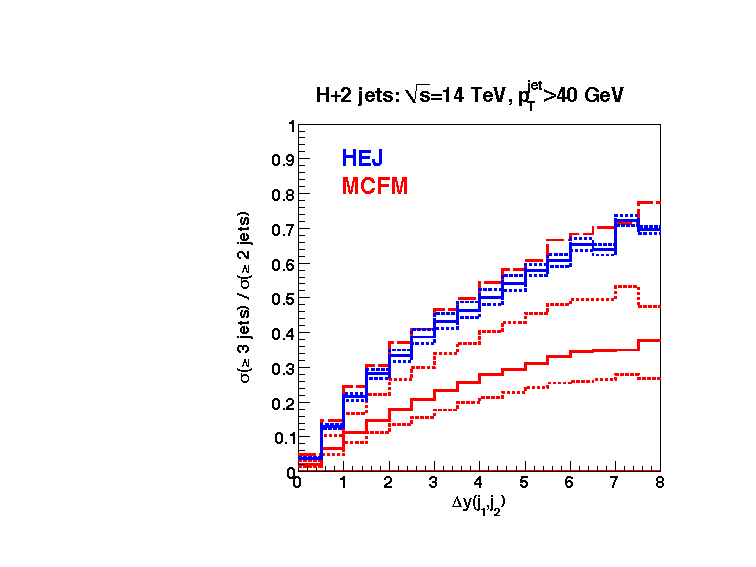
\includegraphics[width=1.0\textwidth]{hJetsRatio1}
				\caption{}
				\label{fig:hJetsRatio1}
			\end{subfigure}
			\captionsetup[subfigure]{oneside,margin={0cm,0cm}}
			\begin{subfigure}[b]{0.48\textwidth}
				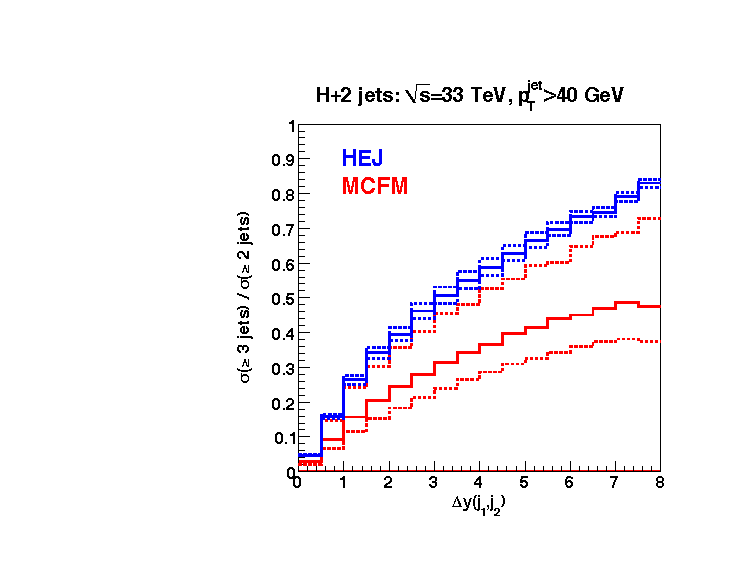
\includegraphics[width=1.0\textwidth]{hJetsRatio2}
				\caption{}
				\label{fig:hJetsRatio2}
			\end{subfigure}
			\begin{subfigure}[b]{0.48\textwidth}
				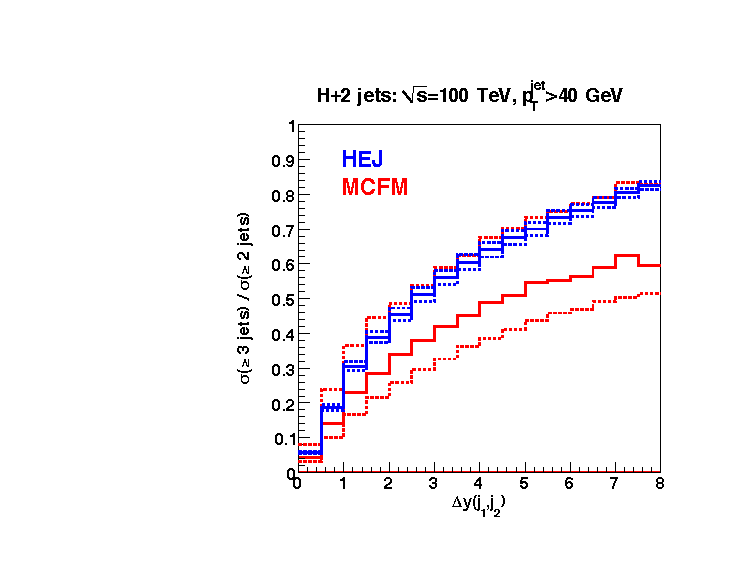
\includegraphics[width=1.0\textwidth]{hJetsRatio3}
				\caption{}
				\label{fig:hJetsRatio3}
			\end{subfigure}

			\caption{The ratio of the inclusive Higgs plus three jet cross-section to inclusive Higgs plus two jet cross-section
			         shown for centre-of-mass energies of $14$TeV (similar to the current LHC), $33$TeV and $100$TeV (possible
			         energy scales for a hadronic future circular collider).}

			\label{fig:higgsratios}
		\end{figure}

		\begin{figure}[hbtp]
			\centering
			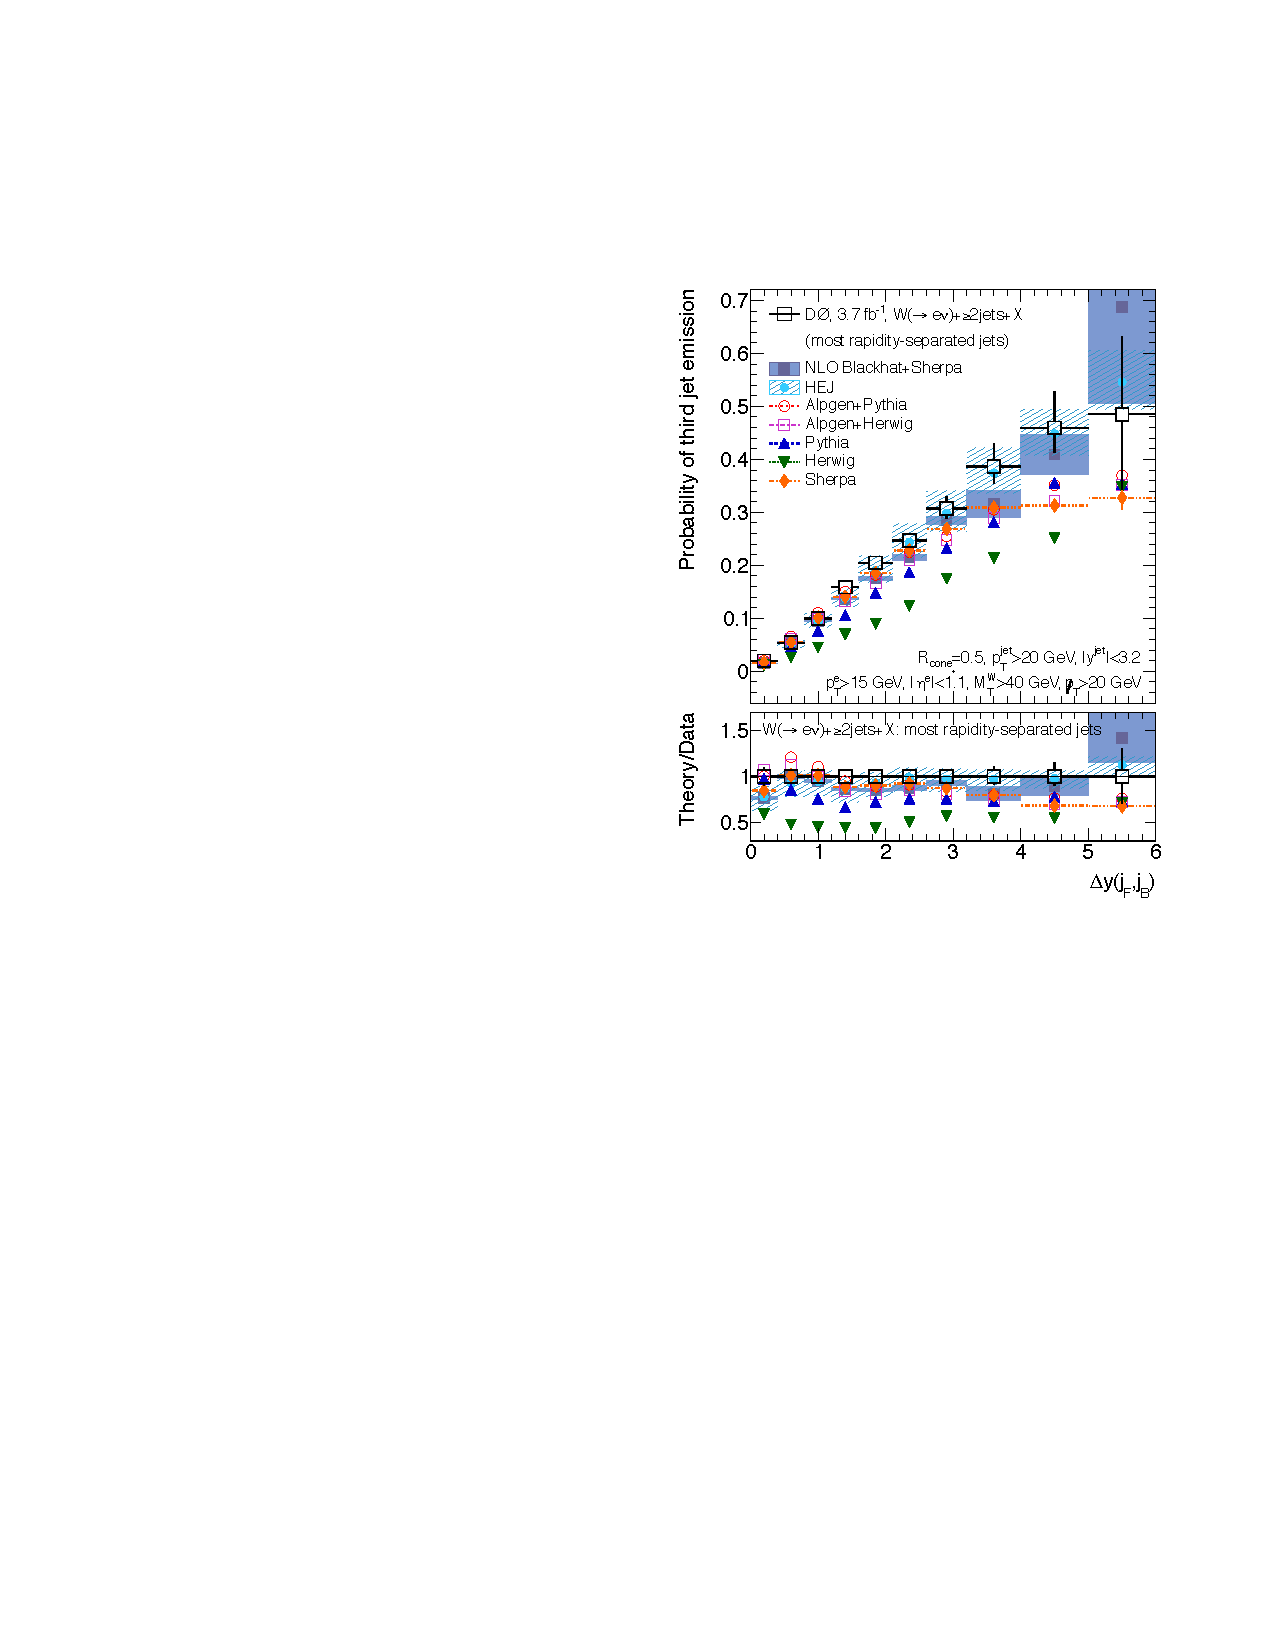
\includegraphics[width=0.75\textwidth]{d0wjets}
			\caption{The probability of a third jet emission in $W^\pm$ plus inclusive dijets as a function of the rapidity gap
			         between the two leading jets in rapidity at the D$\oldemptyset$ experiment at the Tevatron experiment.
			         The data are compared to a number of generators including the leading logarithmic accurate \texttt{HEJ}
			         and the NLO accurate \texttt{Blackhat+Sherpa}.}
			\label{fig:d0wjets}
  		\end{figure}

\section{Spinor-Helicity Notation}
	\label{sec:SpinorHelicity}

	We now move towards the more mechanical aspects of this thesis to discuss a technique which eases calculations.
	In chapters \ref{chap:HEQCD} and \ref{chap:Zs} we choose to work in the spinor-helicity formalism \cite{Dixon:1996wi,CBO9781107706620A004}.
	This is a very convenient choice of notation which allows us to quickly evaluate complicated strings of products of
	Dirac spinors and Dirac matrices which would otherwise be troublesome to work with.\\We begin by looking at the case
	of massless particles; this is relevant for high energy QCD since gluons are massless and the quark masses are often
	negligible compared to the energy scale in a typical scattering process.  The massless Dirac equation can be solved
	by using a plane-wave expansion with some momentum dependent coefficient functions, $u(p)$ and $v(p)$ where $p$ is the
	momentum carried by the particle and must satisfy the on-shell condition $p^2=0$.  This expansion gives the following
	equations:

	\begin{align}
	\begin{split}
		(\slashed p + m)u(p) = 0, \\
		(\slashed p - m)v(p) = 0.
	\end{split}
	\end{align}

	Each of these equations has two independent solutions which we identify as the helicity states, $u^\pm(p)$ and $v^\pm(p)$.
	We use the following notation for these spinors:

	\begin{equation}
		u^\pm(p) = \mid p\pm\rangle, \hspace{1cm} \overline{u^\pm(p)} = \langle p\pm\mid.
	\end{equation}

	In the massless limit we also have the following relation $u^\pm(p) = v^\mp(p)$ which allows us to use the same notation for both
	quarks and anti-quarks.  Often the helicity information will be suppressed in the interests in being concise.  We also define the
	following spinor-brackets:

	\begin{equation}
		\langle pk\rangle = \langle p-\mid k+\rangle, \hspace{1cm} [pk] = \langle p+\mid k-\rangle.
	\end{equation}

	In this language we have the following useful identities:

	\begin{align*}
		\langle ij\rangle[ij] &= s_{ij} & \langle i\pm\mid\gamma^\mu\mid i\pm\rangle &= 2k_i^\mu \\
		\langle ij\rangle &= -\langle ji\rangle & [ij] &= -[ji] \\
		\langle i\pm\mid\gamma^\mu\mid j\pm\rangle\langle k\pm\mid\gamma_\mu\mid l\pm\rangle &=
		2[ik]\langle l j\rangle & \langle k\pm\mid\gamma^\mu\mid l\pm\rangle &=
		\langle l\mp\mid\gamma^\mu\mid k\mp\rangle \\
		\langle i j\rangle\langle k l\rangle &=
		\langle i k\rangle\langle l j\rangle + \langle i l\rangle\langle k j\rangle & [ij][kl] &= [ik][jl]+[il][kj] \\
		\langle i+|\slashed k|j+\rangle &= [ik]\langle kj\rangle & \langle i-|\slashed k|j-\rangle &= \langle ik\rangle [kj]
	\end{align*}

	In the calculations here we use the following convention for spinors.  We express the parton momenta in terms
	of light-cone coordinates where $p^\pm=E\pm p_z$ and $p_{\perp} = p_x + ip_y$.  For outgoing positive (negative) helicity partons,
	$u^+(p)$ ($u^-(p)$) we have:

	\begin{align}
	    u^+(p) &= \begin{pmatrix}
	           \sqrt{p^+} \\
	           \sqrt{p^-}\frac{p_\perp}{|p_\perp|} \\
	           0 \\
	           0 \\
	         \end{pmatrix}\hspace{0.75cm}
	    u^+(p) &= \begin{pmatrix}
	           0 \\
	           0 \\
	           \sqrt{p^-}\frac{p_\perp^*}{|p_\perp|} \\
	           -\sqrt{p^+} \\
	         \end{pmatrix}
	\end{align}

	respectively.  While for incoming positive (negative) helicity partons moving in the positive $z$ direction,
	$u^+(p)$ ($u^-(p)$) we have:

	\begin{align}
	    u^+(p) = \begin{pmatrix}
	           \sqrt{p^+} \\
	           0 \\
	           0 \\
	           0 \\
	         \end{pmatrix}\hspace{0.75cm}
	    u^-(p) = \begin{pmatrix}
	           0 \\
	           0 \\
	           0 \\
	           -\sqrt{p^+} \\
	         \end{pmatrix}
	\end{align}

	respectively.  Lastly for incoming positive (negative) helicity partons moving in the negative $z$ direction,
	$u^+(p)$ ($u^-(p)$) we have:

	\begin{align}
	    u^+(p) &= \begin{pmatrix}
	           0 \\
	           -\sqrt{p^-} \\
	           0 \\
	           0 \\
	         \end{pmatrix}\hspace{0.75cm}
	    u^-(p) &= \begin{pmatrix}
	           0 \\
	           0 \\
	           -\sqrt{p^-} \\
	           0 \\
	         \end{pmatrix}.
	\end{align}

	We also use following form for the Dirac matrices:

	\begin{align}
	    \gamma^0 &= \begin{pmatrix}
	           0 & 0 & 1 & 0\\
	           0 & 0 & 0 & 1\\
	           1 & 0 & 0 & 0\\
	           0 & 1 & 0 & 0\\
	         \end{pmatrix}\hspace{1.2cm}
	    \gamma^1 = \begin{pmatrix}
	           0 & 0 & 0 & -1\\
	           0 & 0 & -1 & 0\\
	           0 & 1 & 0 & 0\\
	           1 & 0 & 0 & 0\\
	         \end{pmatrix}.\\
	    \gamma^2 &= \begin{pmatrix}
	           0 & 0 & 0 & i\\
	           0 & 0 & -i & 0\\
	           0 & -i & 0 & 0\\
	           i & 0 & 0 & 0\\
	         \end{pmatrix}\hspace{0.75cm}
	    \gamma^3 = \begin{pmatrix}
	           0 & 0 & -1 & 0\\
	           0 & 0 & 0 & 1\\
	           1 & 0 & 0 & 0\\
	           0 & -1 & 0 & 0\\
	         \end{pmatrix}.
	\end{align}

	\subsection{Spinor-Helicity Calculations with Massive Partons}
		\label{sub:SMMassive}

		To do calculations with massive partons using the spinor-helicity formalism we must be very careful since all of our favourite
		identities and tricks rely on the spinor brackets, $|i\rangle$, representing massless partons with $p_i^2=0$. We begin by
		defining `fundamental spinors' \cite{spinorThesis} which we can use to build more general spinors and go from there.
		For some $k_0$, $k_1$ satisfying $k_0^2=0$, $k_1^2=-1$ and $k_0\cdot k_1=0$ we can define positive and negative helicity spinors as follows:

		\begin{subequations}
		\begin{align}
			u_{-}(k_0)\overline{u}_-(k_0) &\equiv \omega_- \slashed k_0\\
			u_+(k_0) &\equiv \slashed k_1 u_- (k_0),
		\end{align}
		\label{eqn:definition}
		\end{subequations}

		where $\omega_\lambda = \half(1 + \lambda\gu{5})$ is the helicity projection operator.  In order for these to be valid spinors they must satisfy the following completeness relations:

		\begin{subequations}
			\begin{equation}
				\label{eqn:prop1}
				\sum_\lambda u_\lambda(p)\overline{u}_\lambda(p)=\slashed p + m
			\end{equation}
			\begin{equation}
				\label{eqn:prop2}
				u_\lambda(p)\overline{u}_\lambda (p) = \omega_\lambda\slashed p
			\end{equation}
			\label{eqn:props}
		\end{subequations}

		The spinors in eq. \eqref{eqn:definition} can easily be shown to satisfy these as follows:

		\begin{subequations}
		\begin{align*}
			u_-(k_0)\overline{u}_-(k_0) + u_+(k_0)\overline{u}_+(k_0) &= \omega_-\slashed k_0 + \slashed k_1 u_-(k_0)\overline{u}_-(k_0)\slashed k_1,\\
		        &= \omega_-\slashed k_0 + \slashed k_1 \omega_-\slashed k_0\slashed k_1,\\
		        &= \omega_-\slashed k_0 + \half\gu{\mu}k_{1\mu}(1-\gu{5})\gu{\nu}k_{0\nu}\gu{\sigma}k_{1\sigma},\\
		        &= \omega_-\slashed k_0 + \half k_{1\mu}k_{0\nu}k_{1\sigma}(\gu{\mu}\gu{\nu}\gu{\sigma}-\gu{\mu}\gu{5}\gu{\nu}\gu{\sigma}),\\
		        &= \omega_-\slashed k_0 + \half k_{1\mu}k_{0\nu}k_{1\sigma}(2\gu{\mu}g^{\nu\sigma} - \gu{\mu}\gu{\sigma}\gu{\nu}+2\gu{5}\gu{\mu}g^{\nu\sigma} - \gu{5}\gu{\mu}\gu{\sigma}\gu{\nu}),\\
		        &= \omega_-\slashed k_0 + k_{1\mu}k_{0\nu}k_{1\sigma}\omega_+\gu{\mu}(2g^{\nu\sigma} - \gu{\sigma}\gu{\nu}),\\
		        &= \omega_-\slashed k_0 + 2\slashed k_1 k_0\cdot k_1 - \omega_+\slashed k_1\slashed k_1 \slashed k_0,\\
		        &= \omega_-\slashed k_0 + \omega_+\slashed k_0,
		\end{align*}
		\end{subequations}

		where we have used ${\gu{\mu}, \gu{\mu}}=2g^{\mu\nu}$, ${\gu{\mu}, \gu{5}}=0$ and $\slashed k_1\slashed k_1=k_1^2=0$.
		This proves the property of eq. \eqref{eqn:props} and inserting the definition of $\omega_\lambda$ gives:

		\begin{subequations}
		\begin{align*}
			u_-(k_0)\overline{u}_-(k_0) + u_+(k_0)\overline{u}_+(k_0) &= \half(1-\gu{5})\slashed k_0 + (1+\gu{5})\slashed k_0,\\
			&= \slashed k_0,
		\end{align*}
		\end{subequations}

		which is eq. \eqref{eqn:props} for a massless particle.\\We can use these fundamental spinors
		to form spinors for any given momenta, $p$ (which has $p^2=0$), as follows:

		\begin{equation}
			u_\lambda(p) = \slashed p u_{-\lambda}(k_0) \frac{1}{\sqrt{2p\cdot k_0}},
		\end{equation}

		provided we don't have $p\cdot k_0=0$.  Once again it is easy to show that this spinor satisfies the necessary conditions, for example:

		\begin{subequations}
		\begin{align*}
			u_\lambda(p)\overline{u}_\lambda(p) &= \frac{1}{2p\cdot k_0}\slashed p u_{-\lambda}(k_0)\overline{u}_{-\lambda}(p)\slashed p,\\
			&= \frac{1}{2p\cdot k_0}\slashed p \omega_{-\lambda}\slashed k_0\slashed p,\\
			&= \frac{1}{4p\cdot k_0}\slashed p (1-\lambda\gu{5})\slashed k_0\slashed p,\\
			&= \frac{1}{2p\cdot k_0}p_{\mu}k_{0\nu}p_{\sigma}\omega_{\lambda}\gu{\mu}(2g^{\nu\sigma} - \gu{\sigma}\gu{\nu}),\\
			&= \frac{1}{2p\cdot k_0}\omega_\lambda(2\slashed p p\cdot k_0 - \slashed p\slashed p\slashed k)),\\
			&= \omega_\lambda\slashed p.\\
		\end{align*}
		\end{subequations}

		So far so good.  This can also be generalised so that we can build massive spinors from our fundamental ones.  We can use

		\begin{equation}
			\label{u_def}
			u(q, s) = \frac{1}{\sqrt{2q\cdot k}}(\slashed q + m)u_-(k)
		\end{equation}

		to describe a quark with spin 4-vector $s$, mass $m$ and momentum $q$.  To confirm this we go through the same procedure as above:

		\begin{subequations}
		\begin{align*}
			u_\lambda(p,s)\overline{u}_\lambda(p,s) &= \frac{1}{2q\cdot k_0}(\slashed q + m) u_-(k_0)\overline{u}_-(q)(\slashed q + m),\\
			&= \frac{1}{2q\cdot k_0}(\slashed q + m) \omega_-\slashed k_0 (\slashed q + m), \\
			&= \frac{1}{4q\cdot k_0}(\slashed q + m) (1-\gu{5})\slashed k_0 (\slashed q + m), \\
			&= \frac{1}{4q\cdot k_0}\big[\left(\slashed q \slashed k_0 \slashed q + m\slashed k\slashed q + m\slashed q \slashed
			k_0 + m^2 \slashed k\right)-\gu{5}\left(\slashed q\slashed k\slashed q - m\slashed k\slashed q + m\slashed q\slashed k_0 - m^2\slashed k\right)\big], \\
			&= \half\left(\slashed q + m - \gu{5}\slashed q - m\gu{5} + \frac{m\gu{5}\slashed k\slashed q}{k\cdot q} + \frac{\gu{5}m^2\slashed k}{k\cdot q}\right),\\
			&= \half\left(1+\left(\frac{1}{m}\slashed q - \frac{m}{q\cdot k}\slashed k\right)\gu{5}\right)(\slashed q + m),\\
			&= \half\left(1+\slashed s\gu{5}\right)(\slashed q + m),\\
		\end{align*}
		\end{subequations}

		where the last line defines the spin vector $s = \frac{1}{m} q - \frac{m}{q\cdot k}k$.  Conjecturing
		a similar form for an antiquark spinor with with spin 4-vector $s$, mass $m$ and momentum $q$:

		\begin{equation}
			\label{v_def}
			v(q, s) = \frac{1}{\sqrt{2q\cdot k}}(\slashed q - m)u_-(k)
		\end{equation}

		leads to:

		\begin{subequations}
		\begin{align*}
			v_\lambda(p,s)\overline{v}_\lambda(p,s) &= \frac{1}{2q\cdot k_0}(\slashed q - m) u_-(k_0)\overline{u}_-(q)(\slashed q - m),\\
			&= \half\left(\left(\slashed q - m\right) + \left(-\slashed q + m + \frac{m^2}{q\cdot k_0}\slashed k_0 -
			\frac{m}{q\cdot k_0}\slashed q\slashed k_0 \right)\gu{5}\right), \\
			&= \half\left(1+\slashed s\gu{5}\right)(\slashed q - m).\\
		\end{align*}
		\end{subequations}

		One last check that is worth performing is that these spinors actually satisfy the Dirac equation for both the quark and antiquark case.  For the quark:

		\begin{subequations}
		\begin{align*}
			\slashed q u(q, s) &= \frac{1}{2q\cdot k_0}\slashed q(\slashed q + m)u_-(k_0), \\
			                   &= \frac{1}{2q\cdot k_0}(m^2 + m\slashed q)u_-(k_0). \\
		\end{align*}
		\end{subequations}

		We now define some momentum $\widetilde{q}$ through the relation $q = \widetilde{q} + k_0$ such that $\widetilde{q}^2=0$ and
		$q\cdot k = \widetilde{q}\cdot k$.  Since $q^2=2\widetilde{q}\cdot k=m^2$ we may write

		\begin{subequations}
		\begin{align*}
			\slashed q u(q, s) &= \frac{1}{m}(m^2 + m\slashed q)u_-(k_0), \\
			                   &= (m + \slashed q)u_-(k_0). \\
		\end{align*}
		\end{subequations}

		We can now back substitute from the definition of $u(q, s)$ in eq. \eqref{u_def} to get:

		\begin{subequations}
		\begin{align*}
			\slashed q u(q, s) &= \sqrt{2q\cdot k}u(q, s), \\
			                   &= mu(q,s), \\
		\end{align*}
		\end{subequations}

		which is the Dirac equation for a quark.  The result for antiquarks follows similarly.
		Now we have forms for massive quarks and antiquarks in terms of massless spinors we can
		use all of the spinor-helicity machinery to make our computations more efficient.  Slightly
		more useful forms of equations \eqref{u_def} and \eqref{v_def} can be found by decomposing $q$
		into massless components once again: $q=\widetilde{q}+k$.  Then from eq. \eqref{u_def}:

		\begin{subequations}
		\begin{align*}
			u(q, s) &= \frac{1}{m}(\slashed{\widetilde{q}} + \slashed{k} + m)u_-(k), \\
			        &= \frac{1}{m}\left(\rl{\widetilde{q}^+}{\widetilde{q}^+}k^-\rangle +
			        \rl{\widetilde{q}^-}{\widetilde{q}^-}k^-\rangle + \rl{k^-}{k^-}k^-\rangle +
			        \rl{k^-}{k^-}k^-\rangle + m|k^-\rangle\right), \\
			        &= \frac{[\widetilde{q}k]}{m}|\widetilde{q}^+\rangle + |k^-\rangle,
		\end{align*}
		\end{subequations}

		and similarly for the other helicities and the antiquarks:

		\begin{subequations}
		\begin{align}
			u(q, -s) &= \frac{\langle \widetilde{q}k\rangle}{m}|\widetilde{q}^-\rangle + |k^+\rangle, \\
			v(q,  s) &= \frac{[\widetilde{q}k]}{m}|\widetilde{q}^+\rangle - |k^-\rangle, \\
			v(q, -s) &= \frac{\langle \widetilde{q}k\rangle}{m}|\widetilde{q}^-\rangle - |k^+\rangle
		\end{align}
		\end{subequations}

\section{Monte Carlo Techniques}
	\label{sec:MC}

	\subsection{One Dimensional Integration}
	\label{sub:MCOneD}

	Integrals are ubiquitous in every field of physics and particle physics is no different.  We have already seen many examples where meaningful physical results
	can only be obtained after computing an integral two good examples of this are the convolution of the parton distribution functions with the partonic
	cross-section seen in section \ref{sec:factorisation} and the more complex multi-dimensional integrals seen in section \ref{sub:eg1loop} the calculation
	of the one-loop correction to quark-antiquark production.

	For some of the integrals derived here it is not always feasible (and sometimes not even possible) to calculate them analytically.  In these situations
	we must use a numerical approach to approximate the full result.  Such approaches generally fall into one of two categories; quadrature
	or Monte-Carlo random sampling approaches.  The most appropriate solution depends the integrand itself (and in particular our prior knowledge of
	the integrand) and the number of dimensions we are integrating over.

	Here we briefly consider the one-dimensional case.  Given an integral:

	\begin{equation}
		I = \int_a^b f(x)dx,
		\label{eqn:1DIntegral}
	\end{equation}

	we can use well known results such as the Compound Simpson's Rule to approximate the integral by

	\begin{equation}
		I \approx \frac{h}{3}\sum_{i=0}^{N/2}\left(f(x_{2i-2}) + 4f(x_{2i-1}) + f(x_{2i})\right) + \mathcal{O}(N^{-4}),
		\label{eqn:simpson}
	\end{equation}

	where $N$ is the number of times we have subdivided the integral range $(a, b)$ and $x_i = a + \frac{i(b-a)}{N}$ are the points at which we sample the integrand.
	The error quoted on eq. \ref{eqn:simpson} only shows the dependence on the sampling rate and it should be noted that there are other factors arising
	from the size of the domain of integration and on derivatives of the integrand, $f(x)$.  The $N^{-4}$ scaling of the error in this method makes it a good choice
	for numerics in one-dimension.

	The Monte-Carlo approach to approximating eq. \eqref{eqn:1DIntegral} would be to (pseudo-)randomly select a series of $N$ points, $x_i$, from within the domain of integration
	and then compute the integral as follows:

	\begin{equation}
		I \approx I_{MC} = \frac{b-a}{N}\sum_{i=0}^{N}f(x_i) + \mathcal{O}(N^{-\frac{1}{2}}).
	\end{equation}

	Convergence of this result is assured by the weak law of large numbers (also known as Bernoulli's Theorem) which states that for a series of
	independent and identically distributed random variables, ${X_1,\ldots,X_N}$, each with $\mathbb{E}(X_i) = \mu$ the sample mean approaches the population mean as $N\rightarrow\infty$.
	That is,

	\begin{equation}
		\lim_{N\rightarrow\infty}\frac{X_1+\cdots+X_N}{N}=\mu.
	\end{equation}

	We can see this explicitly since the expectation of $I_{MC}$ under the continuous probability density function $p$ is:

	\begin{align*}
		\mathbb{E}_p[I_{MC}] &= \mathbb{E}_p\left[\frac{b-a}{N}\sum_{i=0}^{N}f(x_i)\right]    \\
		                     &= \frac{b-a}{N}\sum_{i=0}^{N}\mathbb{E}_p\left[f(x_i)\right]    \\
		                     &= \frac{b-a}{N}\sum_{i=0}^{N}\int_{-\infty}^{+\infty}f(x)p(x)dx \\
		                     \intertext{where $p(x)=\frac{1}{b-a}$ is the uniform probability distribution for $x\in(a, b)$.  Hence,}
		\mathbb{E}_p[I_{MC}] &= \frac{b-a}{N}\frac{1}{b-a}\sum_{i=0}^{N}\int_{a}^{b}f(x)dx \\
		                     &= \int_{a}^{b}f(x)dx = I.
	\end{align*}

	Since the convergence of the Monte-Carlo approximation clearly scales significantly worse that the case for quadrature it would seem
	that it is not worth considering and, indeed, for a single dimension it is not. However, the picture changes when we consider
	integrals in dimension $d\geq2$.

	\subsection{Higher Dimensional Integration}
	\label{sub:MCND}

	In the case of higher dimensional integrals e.g.

	\begin{equation}
		I = \int_{[a, b]}f(\vec{x})d\vec{x} = \int_{x_1=a_1}^{x_1=b_1}\cdots\int_{x_n=a_n}^{x_n=b_n}f(x_1, \ldots, x_n)dx_1\ldots dx_n,
	\end{equation}

	we can still look to generalisations of the quadrature methods touched on in section \ref{sub:MCOneD} however the convergence of
	these methods is less favourable.  Quadrature methods have errors which scale with the number of dimensions we are integrating over,
	e.g. $\mathcal{O}(N^{-\frac{4}{d}})$ for the compound Simpson's rule.  We can argue this intuitively since if we have $N$ points in one
	dimension to get an error which scales as $\mathcal{O}(N^{-4})$ then in two dimensions we would require $N^2$ to achieve
	the same density of samplings and hence $N^2\sim\mathcal{O}(N^{-4})\implies N^2\sim\mathcal{O}(N^{-\frac{4}{2}})$ and more generally
	$\mathcal{O}(N^{-\frac{4}{d}})$.

	By comparison the error of a Monte Carlo approximation stays fixed at $\mathcal{O}(N^{-\frac{1}{2}})$ regardless of the number of
	dimensions in the integrals.  We are spared from this so-called `curse of dimensionality' by the Central Limit Theorem
	which states that for a sequence of independent and identically distributed random variables $X_1, \ldots, X_N$ each with
	variance $\sigma^2$ we have:

	\begin{equation}
		\frac{X_1 + \cdots + X_N - N\mathbb{E}(X_1)}{\sqrt{N}\sigma}\xrightarrow{\lim{N\rightarrow\infty}}\mathcal{N}(0, 1),
	\end{equation}

	\noindent where $\mathcal{N}(0, 1)$ is the normal distribution with mean zero and variance 1.  Then using the additive and multiplicative scaling
	of the normal distribution we see that:

	\begin{equation}
		\sum_{i=1}^{N}X_i\xrightarrow{\lim{N\rightarrow\infty}}\mathcal{N}\left(\mu, \frac{\sigma^2}{N}\right),
	\end{equation}

	\noindent where $\mu$ is the mean of the variables $X_i$.  The variance of a normal distribution is well known and we can use this to see that
	for a $d$-dimensional integral we can approximate our uncertainty as:

	\begin{align}
		\int_{[a, b]}f(\vec{x})d\vec{x} &= V\langle f\rangle \pm V\sqrt{\frac{\langle f\rangle^2 - \langle f^2\rangle}{N}}\\
		                                &\equiv V\langle f\rangle \pm V\frac{\sigma_{MC}}{\sqrt{N}},
		\label{eqn:HighDMC}
	\end{align}

	\noindent where $V$ is the volume of the domain of integration, $\langle f\rangle=\sum_i f(x_i)$ and $\langle f^2\rangle=\sum_i f(x_i)^2$.

	\subsection{Variation Reduction Techniques}
	\label{sub:VarReduction}

	In equation~\ref{eqn:HighDMC} we saw that the error estimate of a Monte Carlo approximation depends not only on the number of points sampled,
	$N$, but also on $\sigma_{MC}$.  We can try to reduce $\sigma_{MC}$ by reducing how `variable' the integrand is over the domain of integration, for instance in the extreme
	example where our integrand is $f(x)=f_0$, a constant, it is clear that one Monte Carlo sample is sufficient to compute the integral exactly.
	Previously when computing $\mathbb{E}_p[I_{MC}]$ we used a uniform probability density function but we are free to use any distribution we like
	to perform the integration.  This can be seen since:

	\begin{align*}
		\mathbb{E}_p[I_{MC}] &= \int f(x)p(x)dx, \\
		                     &= \int\frac{f(x)p(x)q(x)}{q(x)}, \\
		                     &= \mathbb{E}_q\left[\frac{I_{MC}p(x)}{q(x)}\right],
	\end{align*}

	\noindent where $q(x)$ is our `importance sampling' distribution.  For example let us consider the integral

	\begin{align}
		I = 150\int_{0}^{\frac{1}{2}}x^2\arcsin x^2dx.
		\label{eqn:simpleIS}
	\end{align}

	The integrand of eq. \ref{eqn:simpleIS} is shown in fig.~(\ref{fig:simpleIS}) along with two potential choices of density functions.
	The uniform distribution (shown in red) will sample the integrand equally across the domain however it is clear from looking
	at the functional form of eq. \ref{eqn:simpleIS} that that isn't the most efficient approach since it is strongly peaked towards the
	right hand side of the domain.  Hence that is where the largest contribution to the Monte Carlo sum will come from.  However if we sample
	the modified integrand using pseudo-random numbers generated from a distribution proportional to $x^4$ (shown in green in fig.~(\ref{fig:simpleIS}))
	we can reduce the variance of our approximation significantly.  Tab. ~\ref{tab:simpleIS} shows how the approximation improves as we vary
	the number of samples, $N$, for the two cases of $q\sim\mathcal{U}(0,0.5)$ and $q\sim x^4$.

	\begin{table}[htp]
		\begin{center}
		\begin{tabular}{c | c | c | c | c}
		$N$       & \multicolumn{2}{c|}{$q\sim\mathcal{U}(0.0,0.5)$} & \multicolumn{2}{c}{$q\sim x^4$} \\ \hline
		          & Approximation & Error       & Approximation & Error       \\ \hline
		$10^1$    & $0.5111428 \pm 1.5932607$ & $0.4318912$ & $0.9424279 \pm 1.6817093$ & $0.0006061$ \\
		$10^2$    & $0.9098668 \pm 2.0212007$ & $0.0331672$ & $0.9429298 \pm 2.6653523$ & $0.0001042$ \\
		$10^3$    & $0.9456974 \pm 2.0415918$ & $0.0026633$ & $0.9431454 \pm 0.8430513$ & $8.936\times10^{-5}$ \\
		$10^4$    & $0.9438040 \pm 2.0222993$ & $0.0007699$ & $0.9430386 \pm 0.2665659$ & $4.504\times10^{-6}$ \\
		$10^5$    & $0.9337252 \pm 2.0040391$ & $0.0093088$ & $0.9430241 \pm 0.0842942$ & $2.848\times10^{-6}$ \\
		\end{tabular}
		\caption{The Monte-Carlo approximation to equation~\ref{eqn:simpleIS} as we vary the number of sampled points, $N$, shown in
		the naive sampling case and in the importance sampled case.}
		\label{tab:simpleIS}
		\end{center}
	\end{table}

	\begin{figure}[htp]
		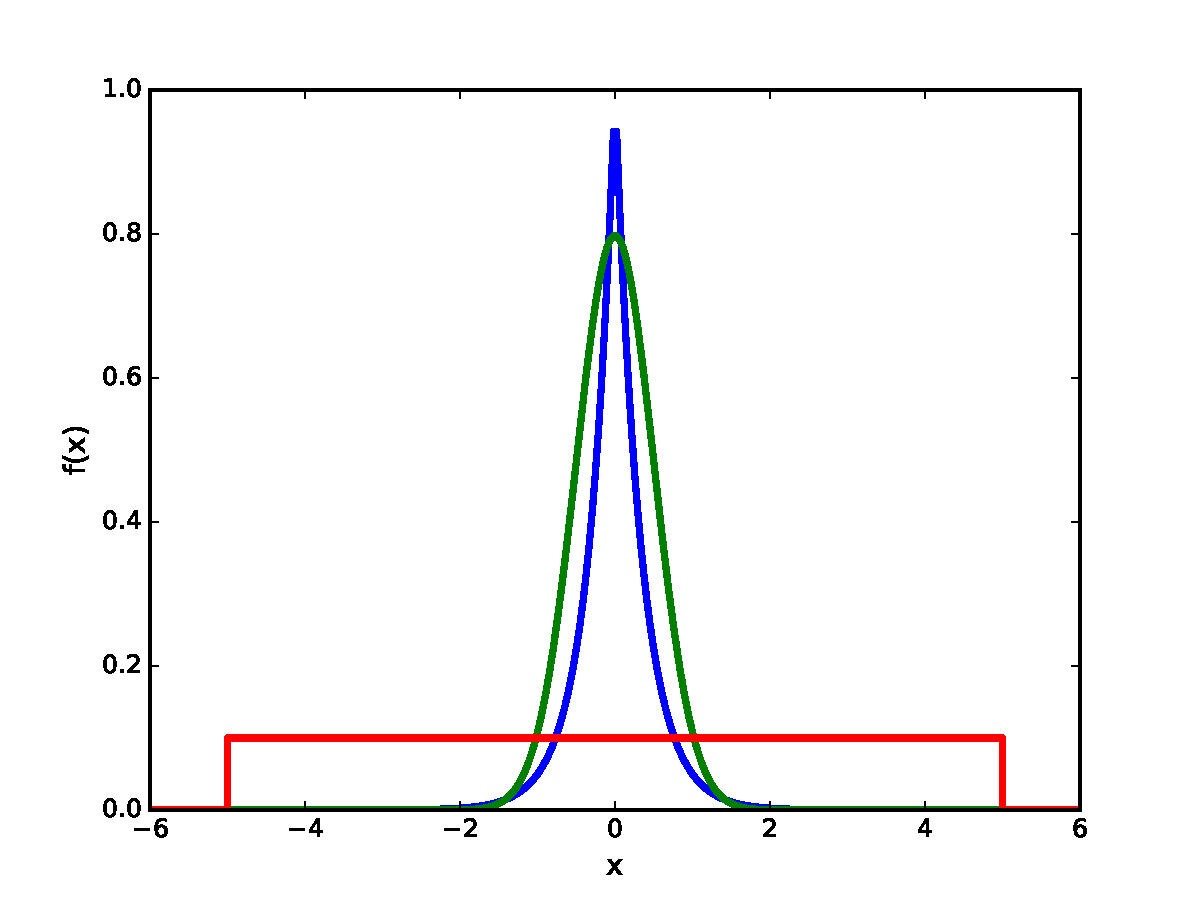
\includegraphics[width=\textwidth]{importanceSampling}
		\caption{A simple importance sampling example (see equation~\ref{eqn:simpleIS}).  The integrand, $f(x)$, is shown in blue,
		the importance sampling distribution is shown in green and, for comparison, the uniform probability density function used
		in the naive case of no importance sampling is also shown (in red).}
		\label{fig:simpleIS}
  	\end{figure}

  	Tab.~\ref{tab:simpleIS} clearly shows the value of an importance sampling approach convergences to the correct result
  	much faster than when we sample uniformly. Of course this tactic relies on us having some prior knowledge of the behaviour of our
  	integrand in order to select the correct probability density function to use which, in more complicated examples is not always
  	possible\footnote{More novel approaches whereby the sampling distribution is modified to improve convergence as the Monte-Carlo
  	iterations are calculated, such as the \texttt{VEGAS} algorithm,
  	exist but they will not be discussed here.}. A more realistic, and relevant, example of importance sampling comes from the
  	cross-section for the production of a $Z^0$ boson in association with dijets.  The matrix element squared for such a process
  	will have following form upon factoring out the $Z^0$ propagator squared:

  	\begin{equation}
  		|\mathcal{M}_{Z^0+jj}|^2 \sim \left|\frac{1}{p_Z^2 - M_Z + i\Gamma_ZM_Z}\right|^2\times f(\text{QCD, EW})\times g(\text{Kinematic}),
  		\label{eqn:schematicZ}
  	\end{equation}

  	where $p_Z$ is the momentum carried by the $Z^0$ boson, $M_Z$ is its mass, $\Gamma_Z$ is its width and $f(\text{QCD, EW})$ will
  	contain all of the coupling information and $g(\text{Kinematic})$ encodes the remainder of the matrix element.  When using a
  	Monte-Carlo approach to generate events of this kind we can use the schematic of \ref{eqn:schematicZ} to \emph{a priori} select
  	an appropriate probability density function to sample from.  Fig. (~\ref{fig:breitWigner}) shows the squared $Z^0$ propagator.
  	Obvious comparisons with fig.~(\ref{fig:simpleIS}) can be drawn in the sense that were we to generate events with a uniform spread
  	of values for $p_Z^2$ we would end with a very slow rate of convergence by oversampling areas where the integrand is very small and slowly varying.

	\begin{figure}[htp]
		\centering
		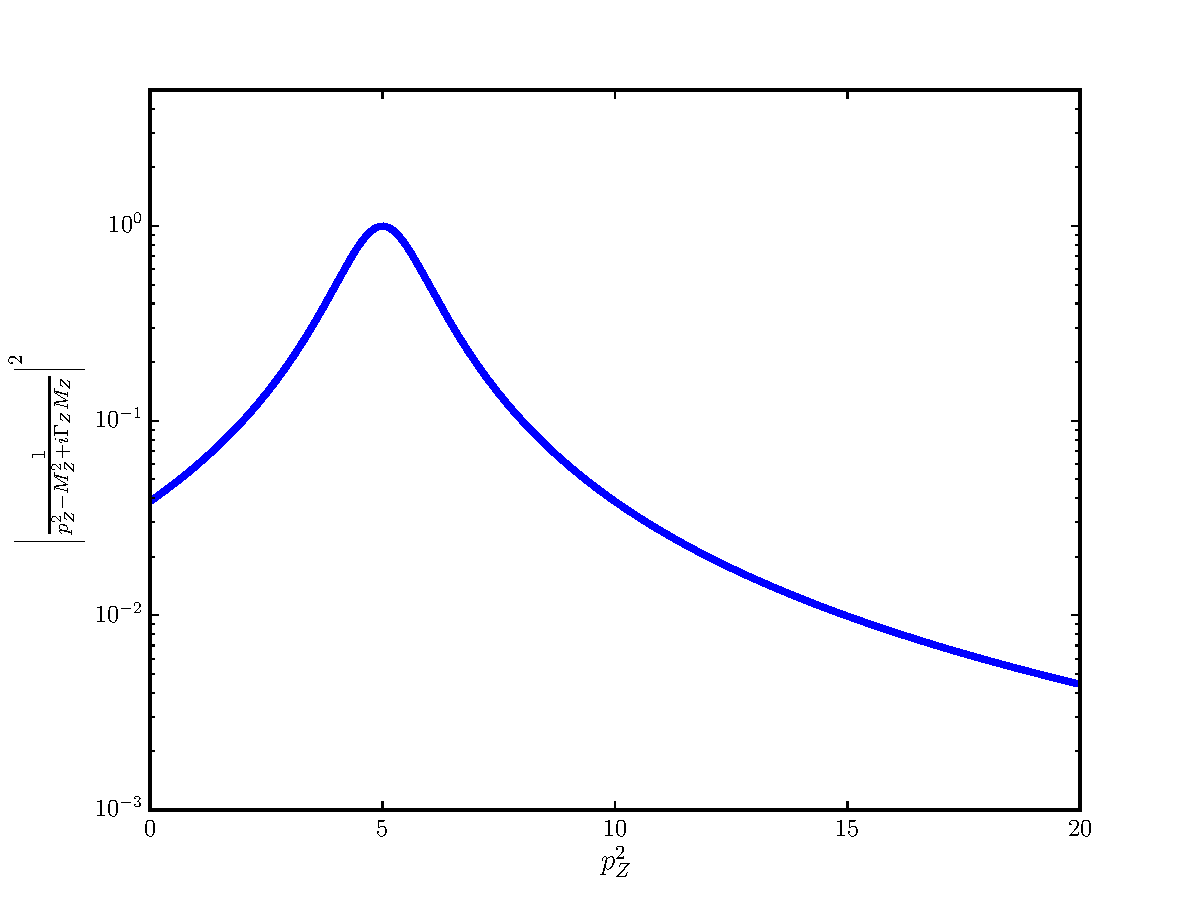
\includegraphics[width=0.8\textwidth, height=0.6\textwidth]{breitWigner}
		\caption{The absolute value squared of the $Z^0$ propagator for a range of values of the invariant mass squared of the
		$Z^0$, $p_Z^2$.  We can see it is strongly peaked at the $Z^0$ mass and, as such, is an ideal candidate for using importance sampling.}
		\label{fig:breitWigner}
  	\end{figure}

	\begin{figure}[htp]
		\centering
		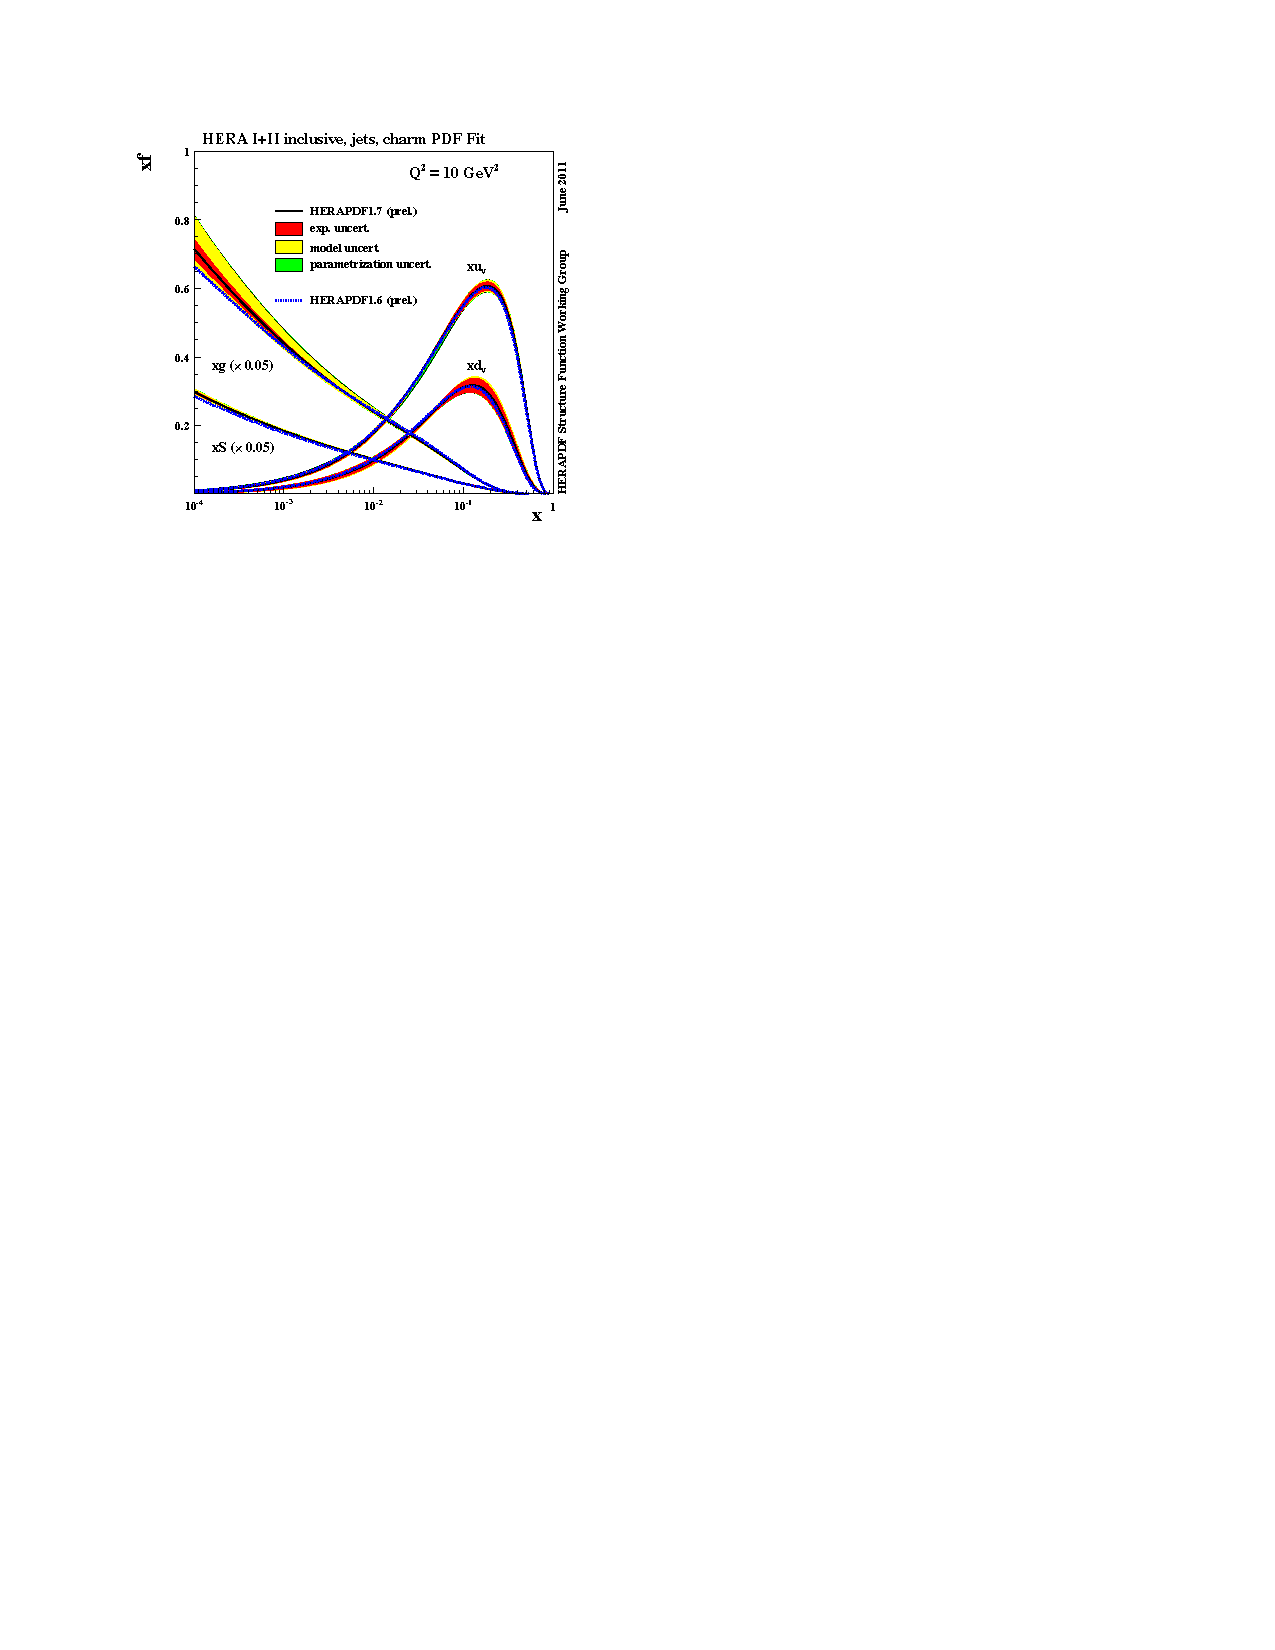
\includegraphics[width=0.8\textwidth, height=0.6\textwidth]{HERAFit}
		\caption{Recent parton distribution function fits from the HERA experiment.  The observed variation in $f(x_{a/b}, Q^2)$, especially at high
		         $x_{a/b}$, can be exploited when computing the equation~\ref{eqn:factorisation} by using an importance sampling approach}
		\label{fig:heraFit}
  	\end{figure}

  	Another good example of importance sampling is found in how we sample the incoming partons in our simulations.  Simple momentum
  	conservation considerations lead us to values for the Bjorken scaling variables of our incoming partons, $x_a$ and $x_b$, and we
  	can use these to intelligently sample the available partons.  The naive way to perform the sum over all possible incoming states
  	would be to uniformly choose a random number corresponding to one of the light quarks, one the light anti-quarks or to a
  	gluon\footnote{Here we mean all except the top and anti-top.  The parton density functions for these are not available
  	and, even if they were, they would be small enough that we could safely ignore their contribution to cross-sections.}.  We can,
  	however, do better than this by using what we know about how the parton density functions vary with $x_{a/b}$ - fig.~(\ref{fig:heraFit})
  	shows this behaviour as measured by the HERA experiment.  By choosing to randomly sample then incoming parton types according to the relative values
  	for the parton density functions we can, once again, reduce the variance of our numerical integrations as much as possible.

